\chapter{Exploratory Study: two months at the primary school}

\label{chap:user_study}

In this chapter I report an \textit{exploratory study} about the usage of tangibles conducted in primary school on upper elementary students. The goals of this study are: collecting evidence that RoomPlaces is able to support a real use case inside a classroom and explore how it is possible to take advantage of tangible user interfaces in order to create new type of learning activities. The research questions of this exploratory study are:

\begin{itemize}
\item How do teachers and learners coordinate their use of shared tangibles?
\item Can the use of tangibles motivates the students? Can the need for coordination of shared tangibles creates opportunities for productive disciplinary engagement? (Engle and Conant \cite{engle:guiding}) Do they become cultural artifacts (a la Horn \cite{horn:role})?
\end{itemize}

The research questions are intentionally grouped in two sets: the first one is about the mechanisms that students use for access to the tangibles, the second is about the effective benefits that tangibles give to the learning experience.

In order to develop the software application used for this study, \textit{RoomPlaces} was used in combination with \textit{nutella} framework for building an interactive ecosystem simulation called WallCology that is a well known \textit{Embedded Phenomena} invented by Moher \cite{moher:wallcology}. The application was written from scratch using the capabilities of nutella and RoomPlaces for rapidly developing the final prototype.

In the next sections I explain the context in which the study is conducted, how WallCology was built with an emphasis on how RoomPlaces was used to support the study, the method that I used for collecting and analyzing data and the results obtained in this study.

\section{Context description}
WallCology study was run in parallel in three classes, of 16 primary school students each, for two months. Every class worked on its own state of the simulation: as other \textit{Embedded Phenomena}, \textit{WallCology} has a state in every time instant, also when the students cannot observe it. This state is represented by the number of creatures present in a certain ecosystem. There was no contact at all between classes, the same activities were done in all the classes in order to compare the outcomes.

\subsection{WallCology}
The version of WallCology implemented for this user study is an improvement of the original prototype presented in 2008 because the technology used for developing it is more advanced and knowledge from the previous study was used in order to improve the user experience. WallCology is a virtual ecosystem \textit{simulated investigation} that runs continuously from the first day until the last that is used. The uniqueness of this \textit{Embedded Phenomena} is in the used metaphor: eleven different species of creatures live inside the walls of the classroom, they populate the entire wall and small parts of them are made visible using virtual tools called \textit{Wallscopes} made with a PC running a computer graphic simulation shown in \ref{fig:ecosystem_1}. 

\begin{figure}
\centering
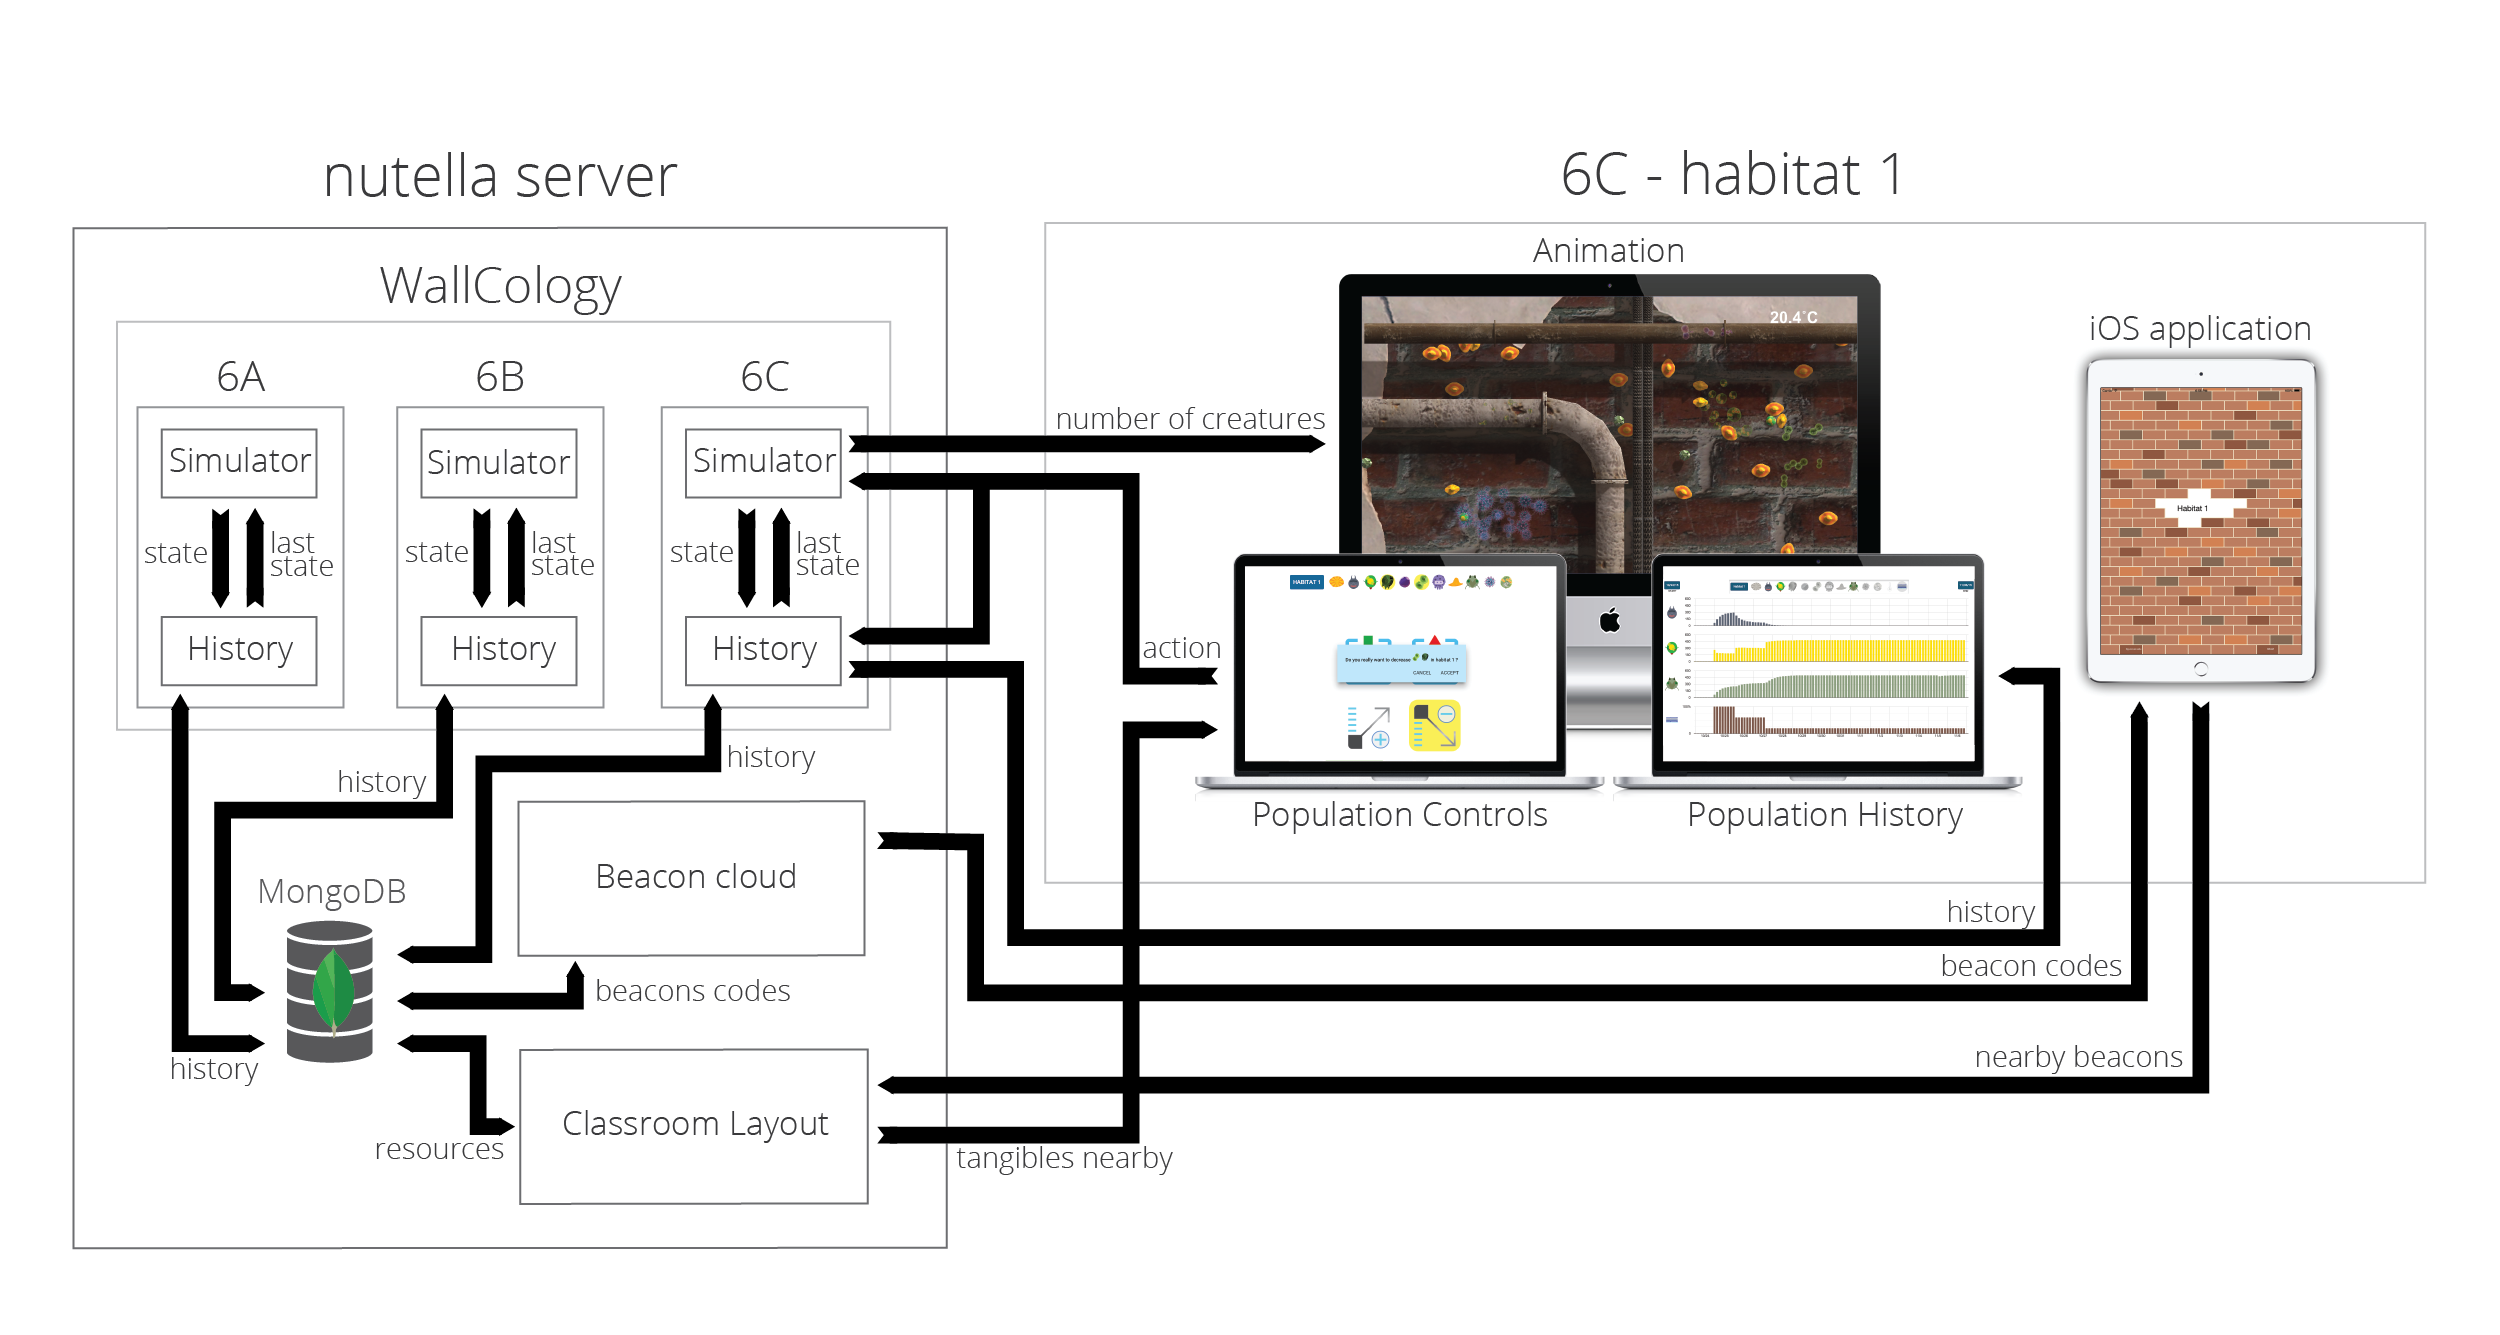
\includegraphics[width=6in]{images/wallcology-structure.png}
\caption{WallCology application structure}
\label{fig:wallscopes}
\end{figure}

In order to have quantitative information about the species that live inside the walls there's another interface tool called \textit{History Graphs}: it displays how the species populations evolve overtime in a certain habitat. The simulation runs all the time and the changes happen slowly when students are not watching the \textit{Wallscopes} (for example during the night). This tool capture the history of the population that evolve overtime and allows students to explore, for any point in time, how many creatures were in a certain habitat. The tool is shown in \ref{fig:population_history}.

The third interface is the \textit{Population Control} and allow students and teachers to interact and modify the environments, changing the population levels and the habitat variables (like the number of pipes present or the temperature). The interface is visible in \ref{fig:population_controls_unlocked}.
There are four actions allowed on the species:
\begin{itemize}
    \item Increase: increment the creatures of a certain species.
    \item Decrease: reduce the creatures of a certain species.
    \item Insert: inject a new species that was not present before.
    \item Remove: eliminate completely all the elements of a species.
\end{itemize}

There are four actions that can change the habitat:
\begin{itemize}
    \item Temperature increase.
    \item Pipe collapse.
    \item Wall collapse.
    \item Infestation of a foreign species.
\end{itemize}

The environmental actions are reserved for the teacher and the species actions can be executed by students and called \textit{perturbations}. The tangible controls were introduced in order to allow students to execute those actions and the tangible interface is proposed as an alternative to the traditional web interface that was also present. Both the interfaces were explained to children and look exactly the same with the only difference that when tangibles were enabled the cursor on the screen was disabled. This interface employs \textit{RoomPlaces} APIs, implemented in \textit{nutella.location}, in order to check if some tangible is present around the \textit{Wallscopes} (it was decided a threshold distance of 70 centimeters, below it an enter event is dispatched and the interface reacts to that action).

\begin{figure}
\centering
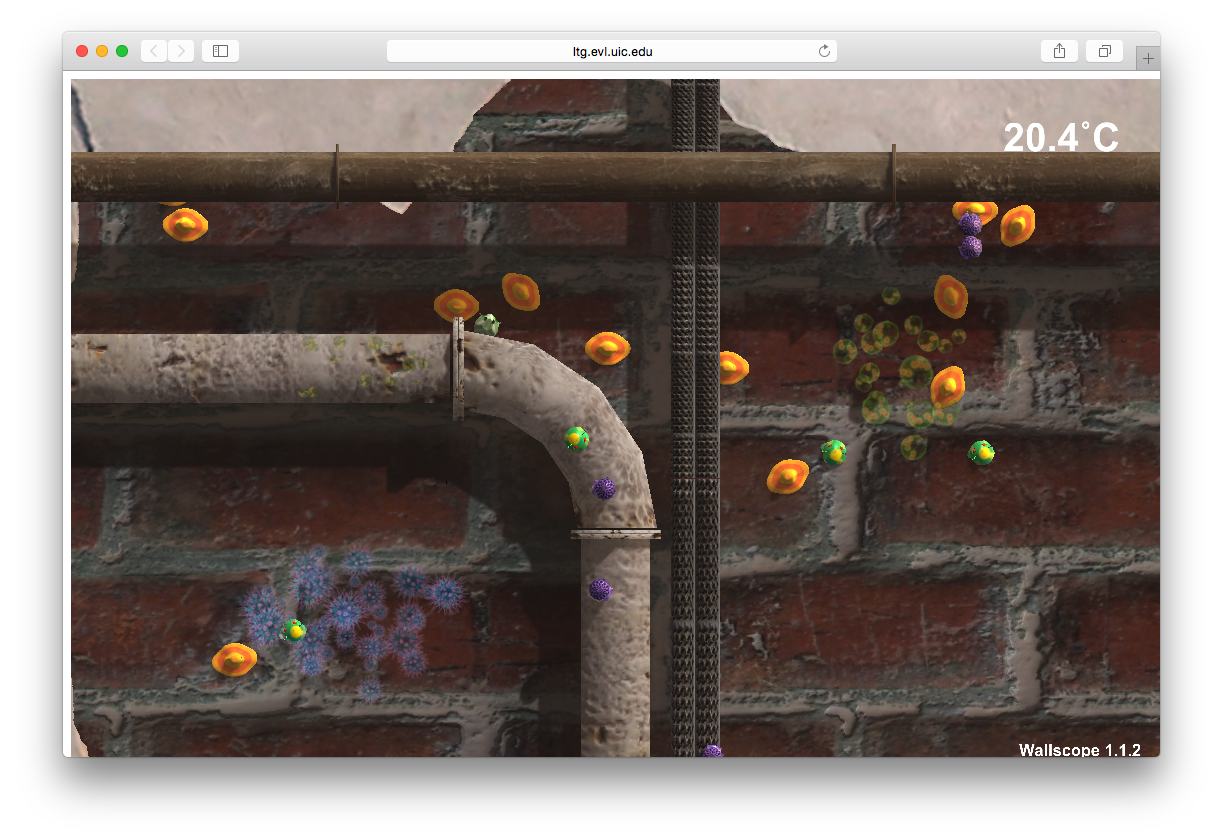
\includegraphics[width=5in]{images/ecosystem-1.png}
\caption{Habitat Simulation Interface}
\label{fig:ecosystem_1}
\end{figure}

All the interfaces earlier introduced are nutella interfaces and implemented using nutella library.

\subsection{Hardware components}
Every habitat is a physical place inside the classroom, where is present a computer that represents the WallScope and a tablet that senses if there are tangibles near that habitat. At the beginning of every lesson, they are both started and manually configured for the classroom. In order to do this initial configuration, it was used \textit{RoomCast} software component, that embeds all the functions for selecting the class and the ecosystem number.

Physical tangibles were created using a 3D printer and later painted for representing exactly the creatures inside the simulation.

\subsection{Population controls interface}
\label{subsec:population_control_interface}

The function of this interface is applying perturbations to the habitats. The interface takes the habitat number as parameter and uses it for knowing what is the resource identifier (rid) of the tablet that is tracking tangibles for that habitat. Once the resource identifier is known, the interface invokes the events APIs contained in \textit{nutella.location} module (that provides a push functionality) asking to be notified every time a tangible enters or exits the habitat. The role of \textit{RoomPlaces APIs} is fundamental in this scenario because they allow to decouple the two hardware components, giving advantages compared to a Client-Server model that requires the server to be reliable and willing to accept connections every time. The improvements are:
\begin{itemize}
    \item The interface on the computer and the application on the tablet can be started independently, there's no predefined order.
    \item One of the two components can be replaced real time if necessary (e.g. a tablet out of battery can be replaced with another one) without impacting the second component.
    \item In case of network problems it is sufficient to reconnect the components to Internet.
\end{itemize}

The interface has two states: \textit{locked} (\ref{fig:population_controls_locked}) and \textit{unlocked} (\ref{fig:population_controls_unlocked}). By design this interface doesn't allow any interaction with the mouse and it is unlocked only when a \textit{tangible key} is present near the habitat (detected with the tablet). On the top part of the interface is present the species selector that shows in every moment the species that are selected. On the bottom there are the four actions: insert, remove, increase, decrease. 

In order to execute one action on an habitat at least three tangibles must be detected by the tablet:
\begin{itemize}
    \item Species tangible: one or more species on which execute the action
    \item Action tangible: the action that must be executed on the selected species
    \item Key tangible: unlock the interface
\end{itemize}
Once all those elements are present, a confirmation message is displayed and the action is sent to the simulation bot (using \textit{nutella.net} APIs) that will update the simulation state.

There are a couple of features that are present in the interface and are the result of functionalities provided by RoomPlaces. When the interface is first started, it is unknown if there are tangibles inside the habitat (entering events are sent before the interface starts are lost), for this reason the first action executed during the bootstrap is discovering (using RoomPlaces APIs contained in \textit{nutella.location}) if some tangible is in proximity of the tablet (\textit{pull} functionality). When the key leaves the habitat, the interface is automatically locked and the species and actions automatically deselected and when it re-enters the habitat the pull functionality is used again in order to check which species and action to select. It is important to highlight that every time the push functionality is used the result is instantly returned without asking the server, this mechanism speeds up the interface and creates a better user experience. During the activity, this interface was improved in order to prevent some type of error that students committed in the early lessons. A confirmation message was added when an action was executed on the server, this message is useful for being sure that the server is still working (no crash occurred) and is useful for the students because they can be sure that the action is registered in the system.

\begin{figure}
\centering
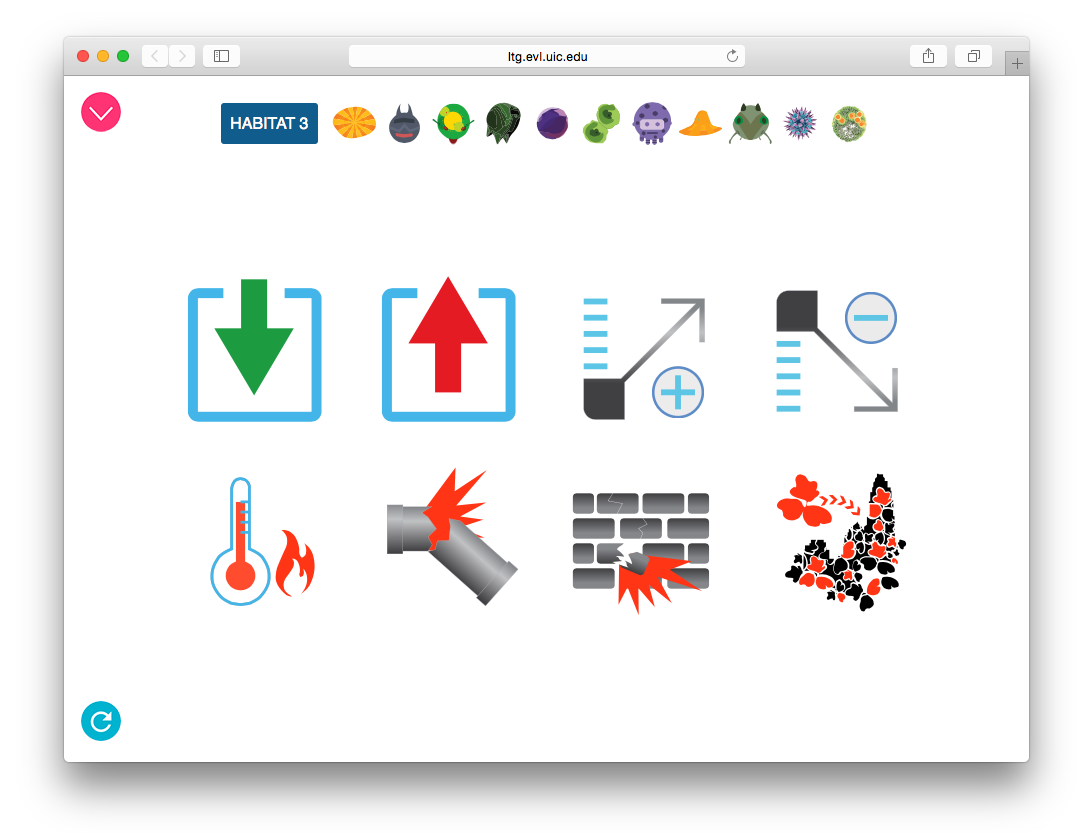
\includegraphics[width=4.5in]{images/population-controls-teacher.png}
\caption{Complete population controls interface for teachers}
\label{fig:population_controls_teachers}
\end{figure}

\begin{figure}
\centering
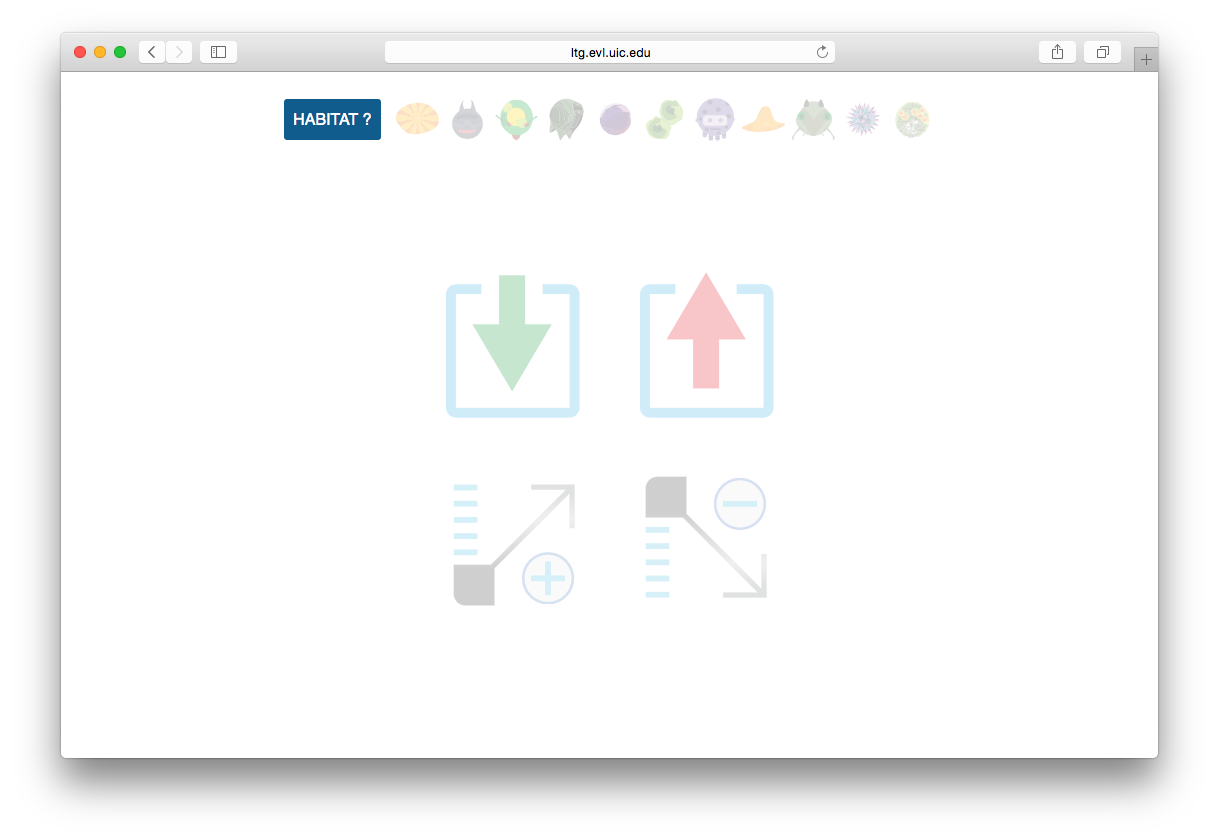
\includegraphics[width=4.5in]{images/population-controls-locked.png}
\caption{Population controls interface locked}
\label{fig:population_controls_locked}
\end{figure}

\begin{figure}
\centering
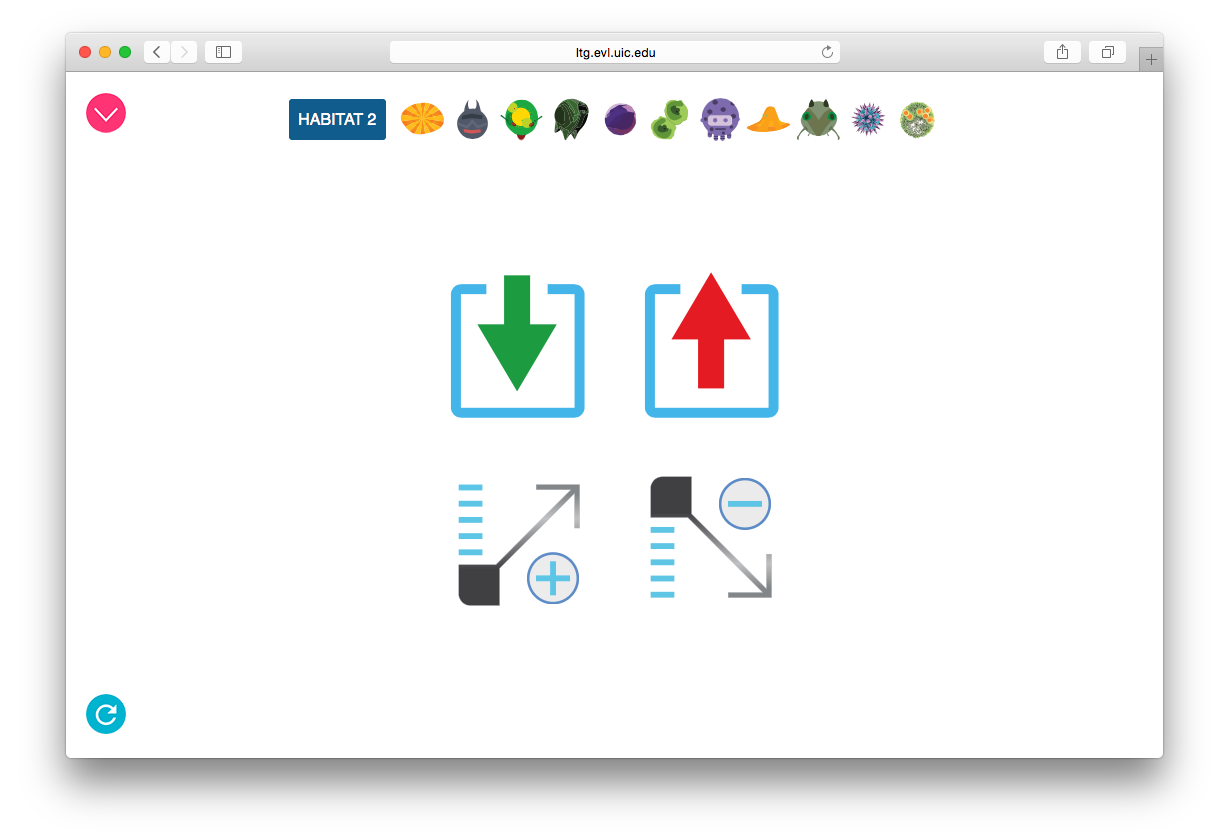
\includegraphics[width=4.5in]{images/population-controls-unlocked.png}
\caption{Population controls interface unlocked}
\label{fig:population_controls_unlocked}
\end{figure}

\begin{figure}
\centering
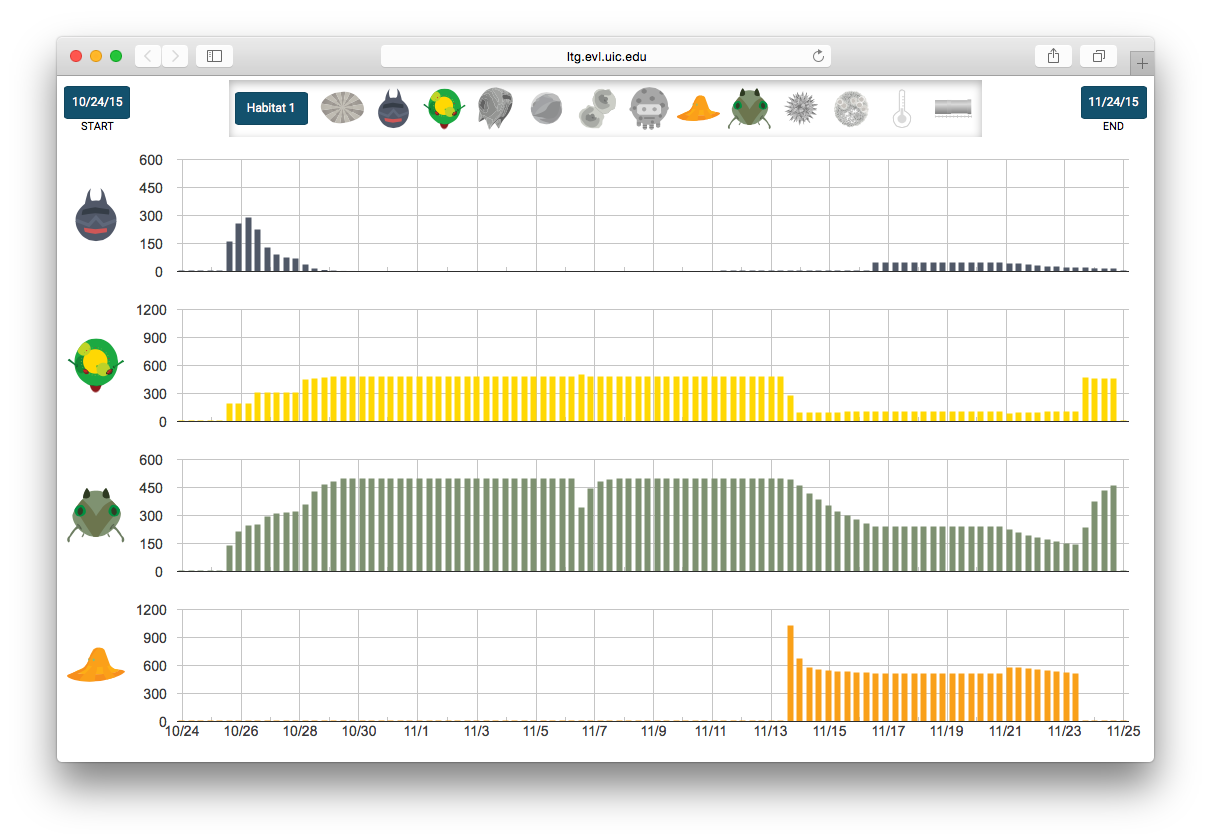
\includegraphics[width=4.5in]{images/population-history.png}
\caption{Population history tool}
\label{fig:population_history}
\end{figure}

\subsection{RoomPlaces configuration}
In order to provide the best user experience possible, it is necessary to hide all the technical details about how tangibles work, at the point in which the user cannot feel that they contain an electronic device while using them. In order to do it, I took advantage of the different levels of abstraction between the hardware device (the iBeacon) and the \textit{population controls} interface. In the next paragraphs I describe those abstractions and why they are important.

The first abstraction layer is provided by \textit{Beacon Cloud}. Every beacon used in the study was manually inserted in the list (only once when it was purchased) and an human readable name was assigned to it. It is possible to see a list of beacons in \ref{fig:wallcology_beacon_cloud}. This abstraction is important because iBeacons have three identifiers that are too long to be remembered (they're long because every beacon must be unique in the world), associating a human readable name considerably increase the usability of \textit{Classroom Layout} interface minimizing the errors end the time during the developing phase.

\begin{figure}
\centering
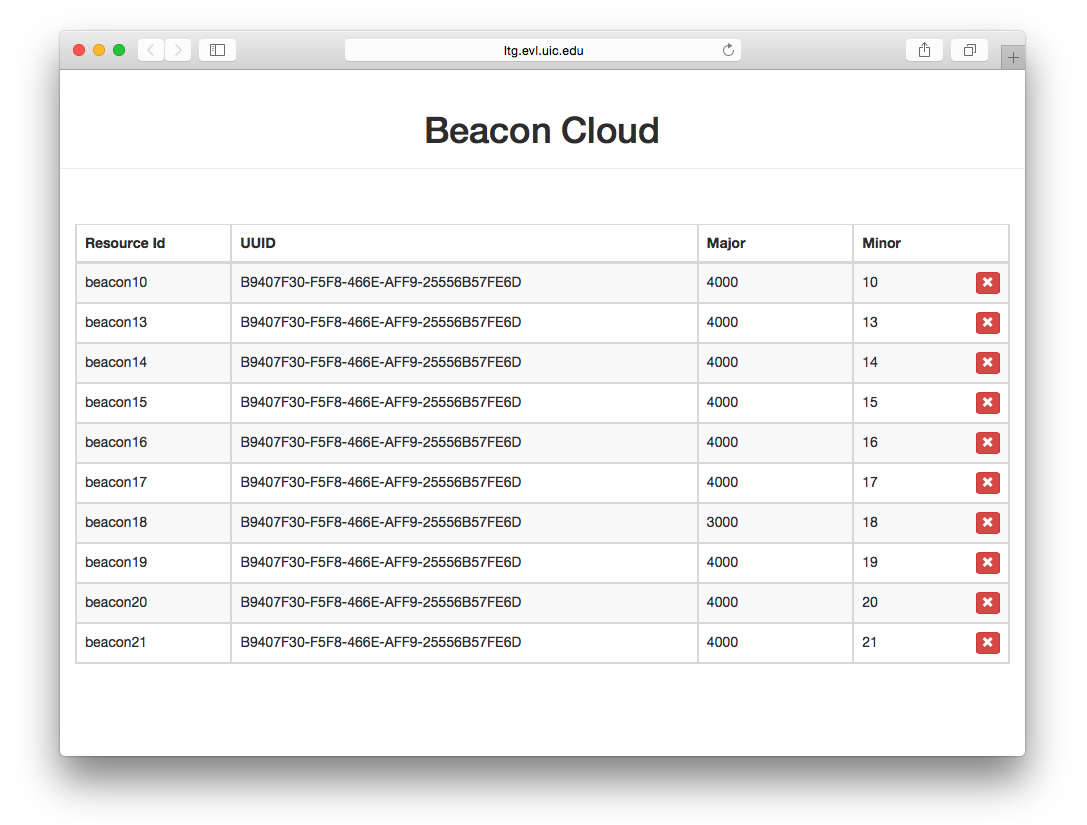
\includegraphics[width=4.5in]{images/wallcology-beacon-cloud.png}
\caption{Beacon Cloud configuration phase}
\label{fig:wallcology_beacon_cloud}
\end{figure}

The second layer of abstraction is provided by \textit{Classroom Layout} component: all the beacons are inserted in automatic \textit{proximity} tracking mode, and for every beacon, additional information was associated to it: the role (key, action or species) and an alphanumeric identifier (the species index or the action name). This abstraction is particularly useful in case of hardware failure of beacons (that can happen due to the battery depletion): it introduces redundancy because the same role can be assigned to more than one beacon and if the first one fails it can be quickly replaced. \textit{Population control} interface has only to look at the "role" data associated with the object and to "key", "action" or "species" data for discovering all the information about the tangible, without the need to hard-code beacon identifiers in the interface. During the Classroom Layout configuration, 19 \textit{tangibles} were introduced as dynamic resources (11 species, 4 actions and 4 keys) and 4 \textit{Wallscopes} as static resources (able to track the dynamic resources) with a proximity radius of 70 centimeters. This configuration was repeated for all the three classes.

\begin{figure}
\centering
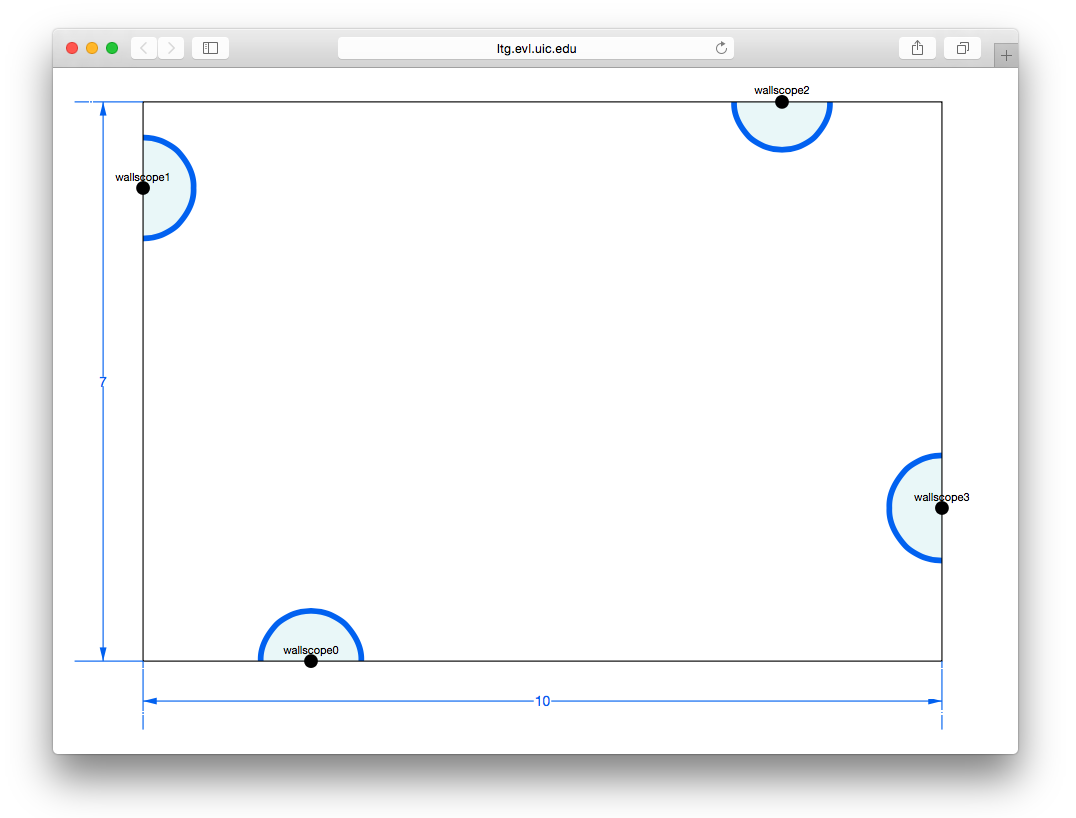
\includegraphics[width=4.5in]{images/wallcology-classroom-layout.png}
\caption{Population controls interface unlocked}
\label{fig:wallcology_classroom_layout}
\end{figure}

The last action that enabled the integration of tangibles is initializing \textit{nutella.location} module (RoomPlaces APIs) inside \textit{population control} interface with the right wallscope resource identifier in order to virtually connect the tablet to the \textit{population control} interface.

\subsection{Wallcology iPad application}
It is a simple application that uses the \textit{nutella.location} module encapsulated in an iOS framework in order to be easy to integrate in an iOS application written in Swift. The application displays a simple user interface that allows to choose the class name and the identifier to use (\textit{Wallscope} index).

Even if this application was very easy to write and deploy, it is the core of the \textit{RoomPlaces} mechanism and everything that happen behind the scenes is encoded in the nutella.location module integrated in nutella\_lib.swift \cite{nutella_lib_swift}. The application communicates with Beacon Cloud and downloads all the information about beacons. When it has the list, starts sensing for every beacon around it and in case iOS discovers some one of them, reports the \textit{resource identifier} to \textit{Classroom Layout} bot that knows the configuration of the classroom and can decide if a proximity event must be dispatched.

\begin{figure}
\centering
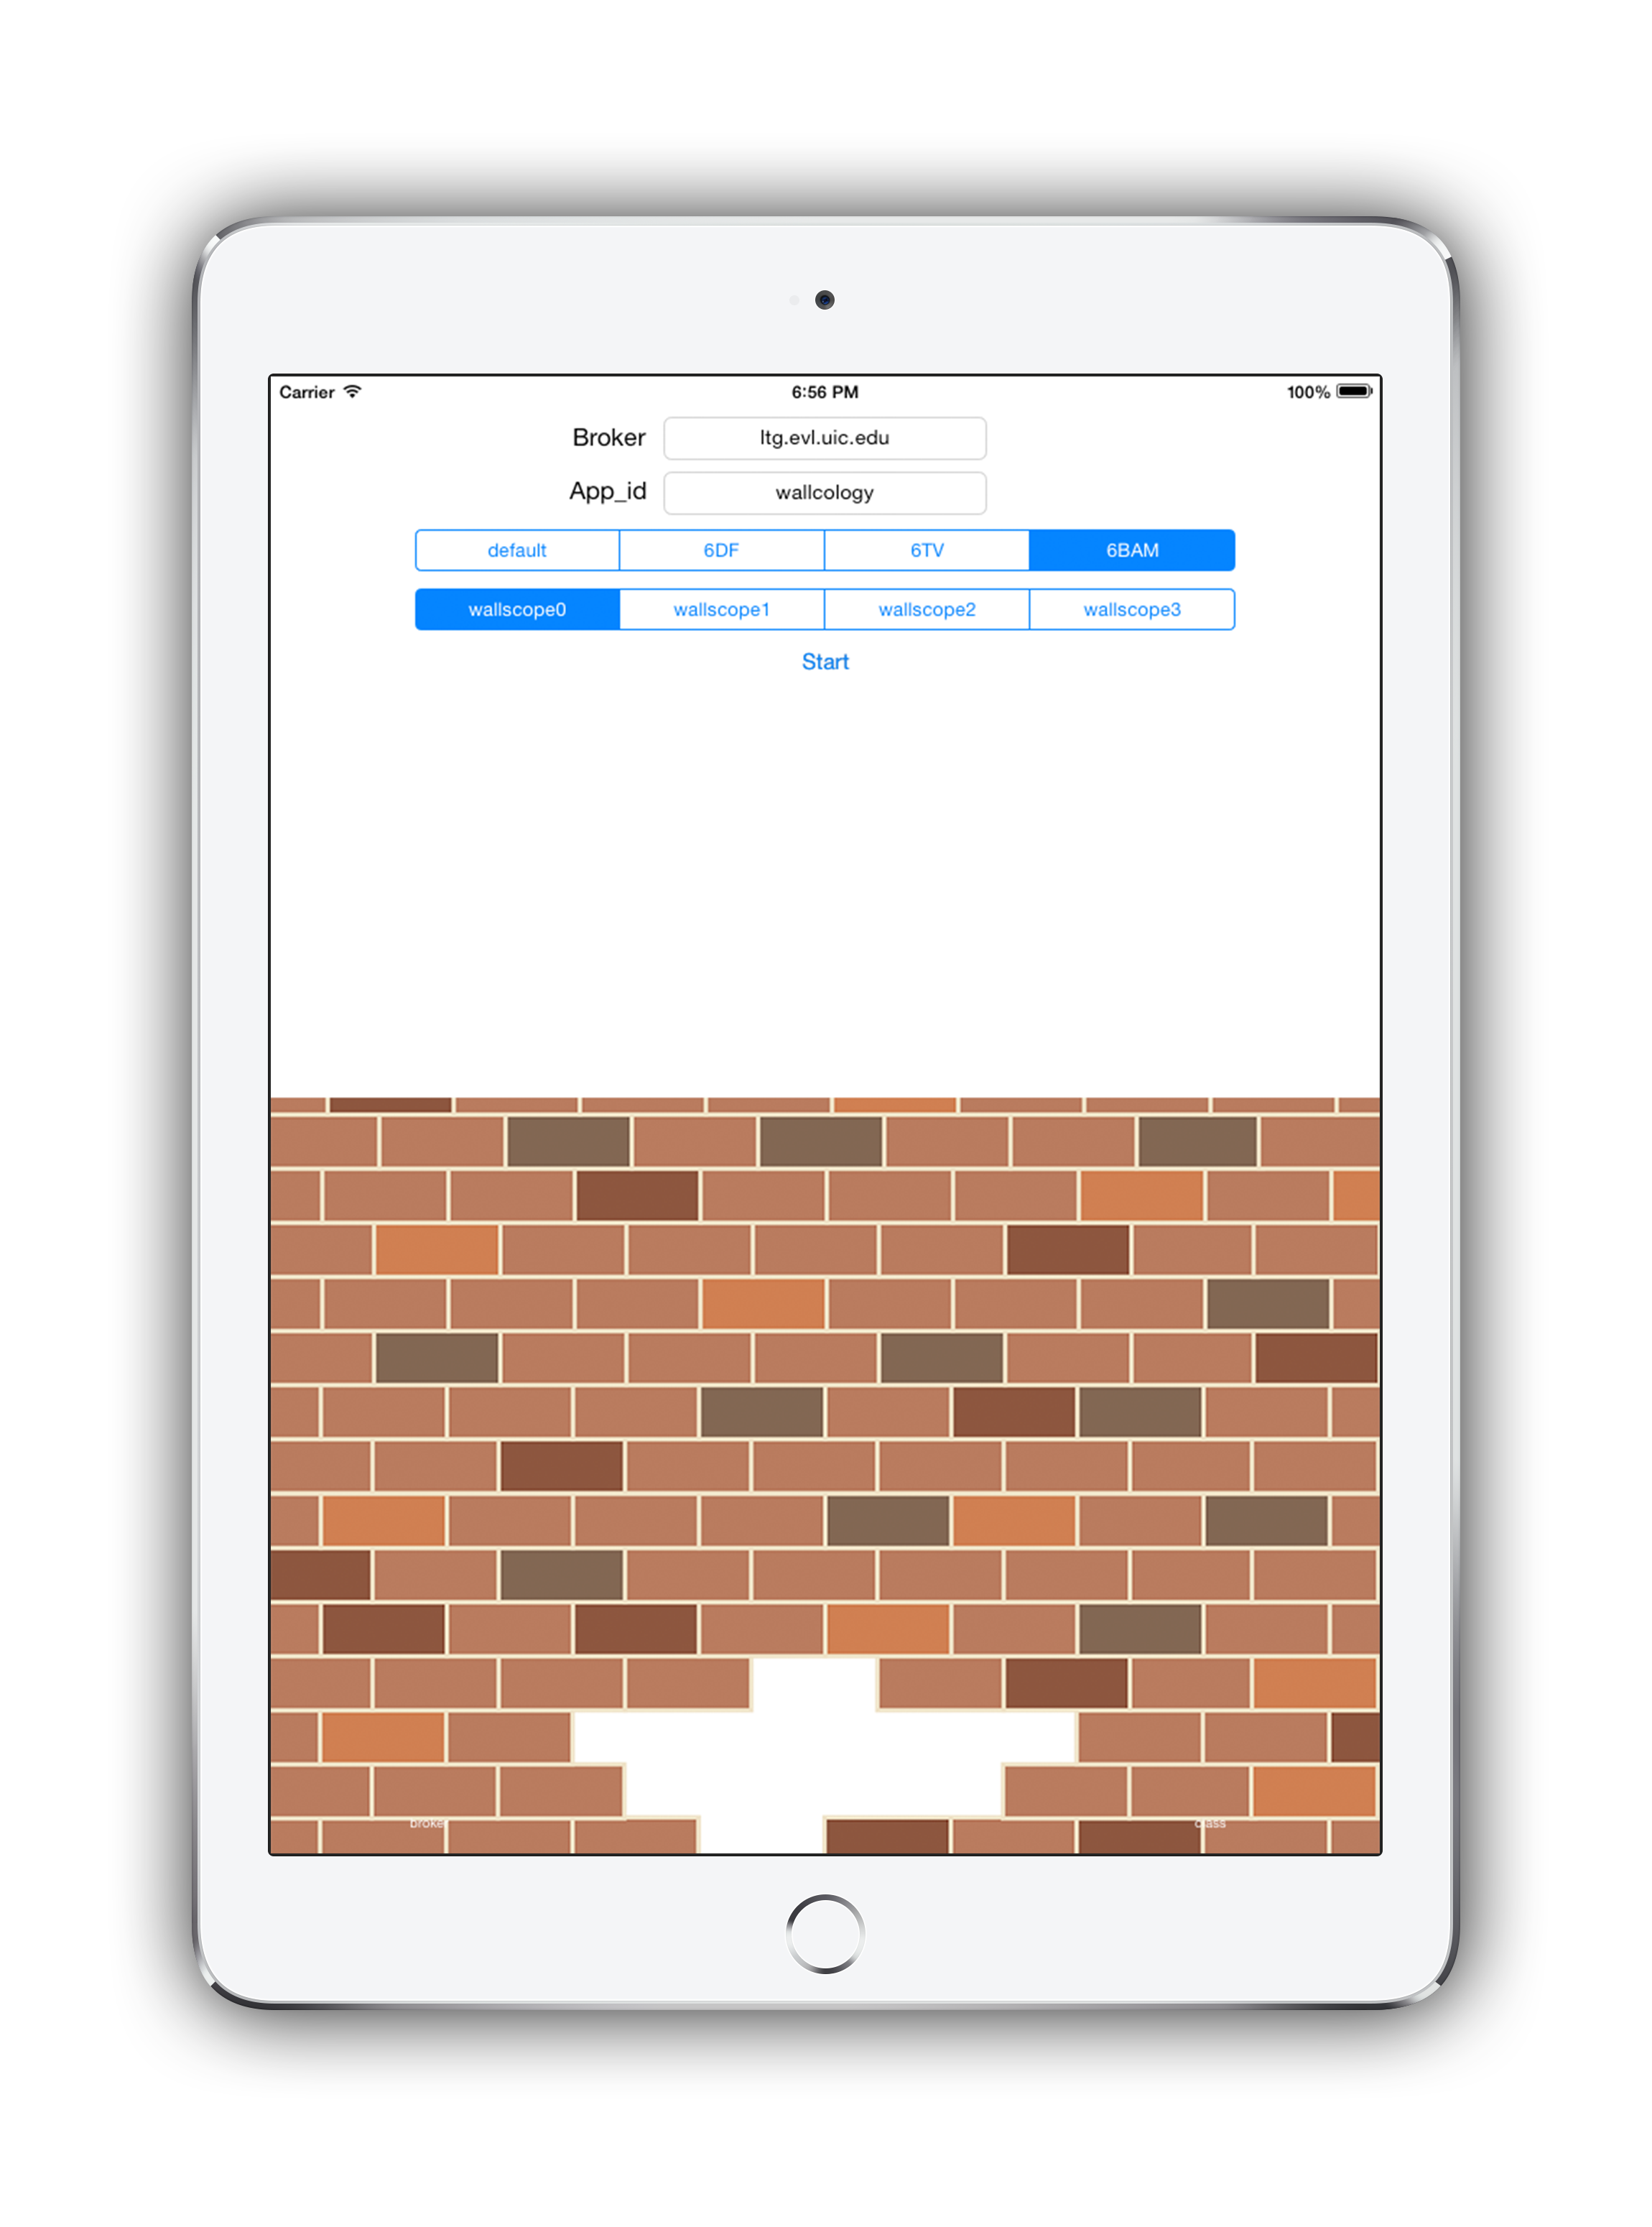
\includegraphics[width=3in]{images/wallcology-ios.png}
\caption{iOS application configuration phase}
\label{fig:wallcology_ios_config}
\end{figure}

\begin{figure}
\centering
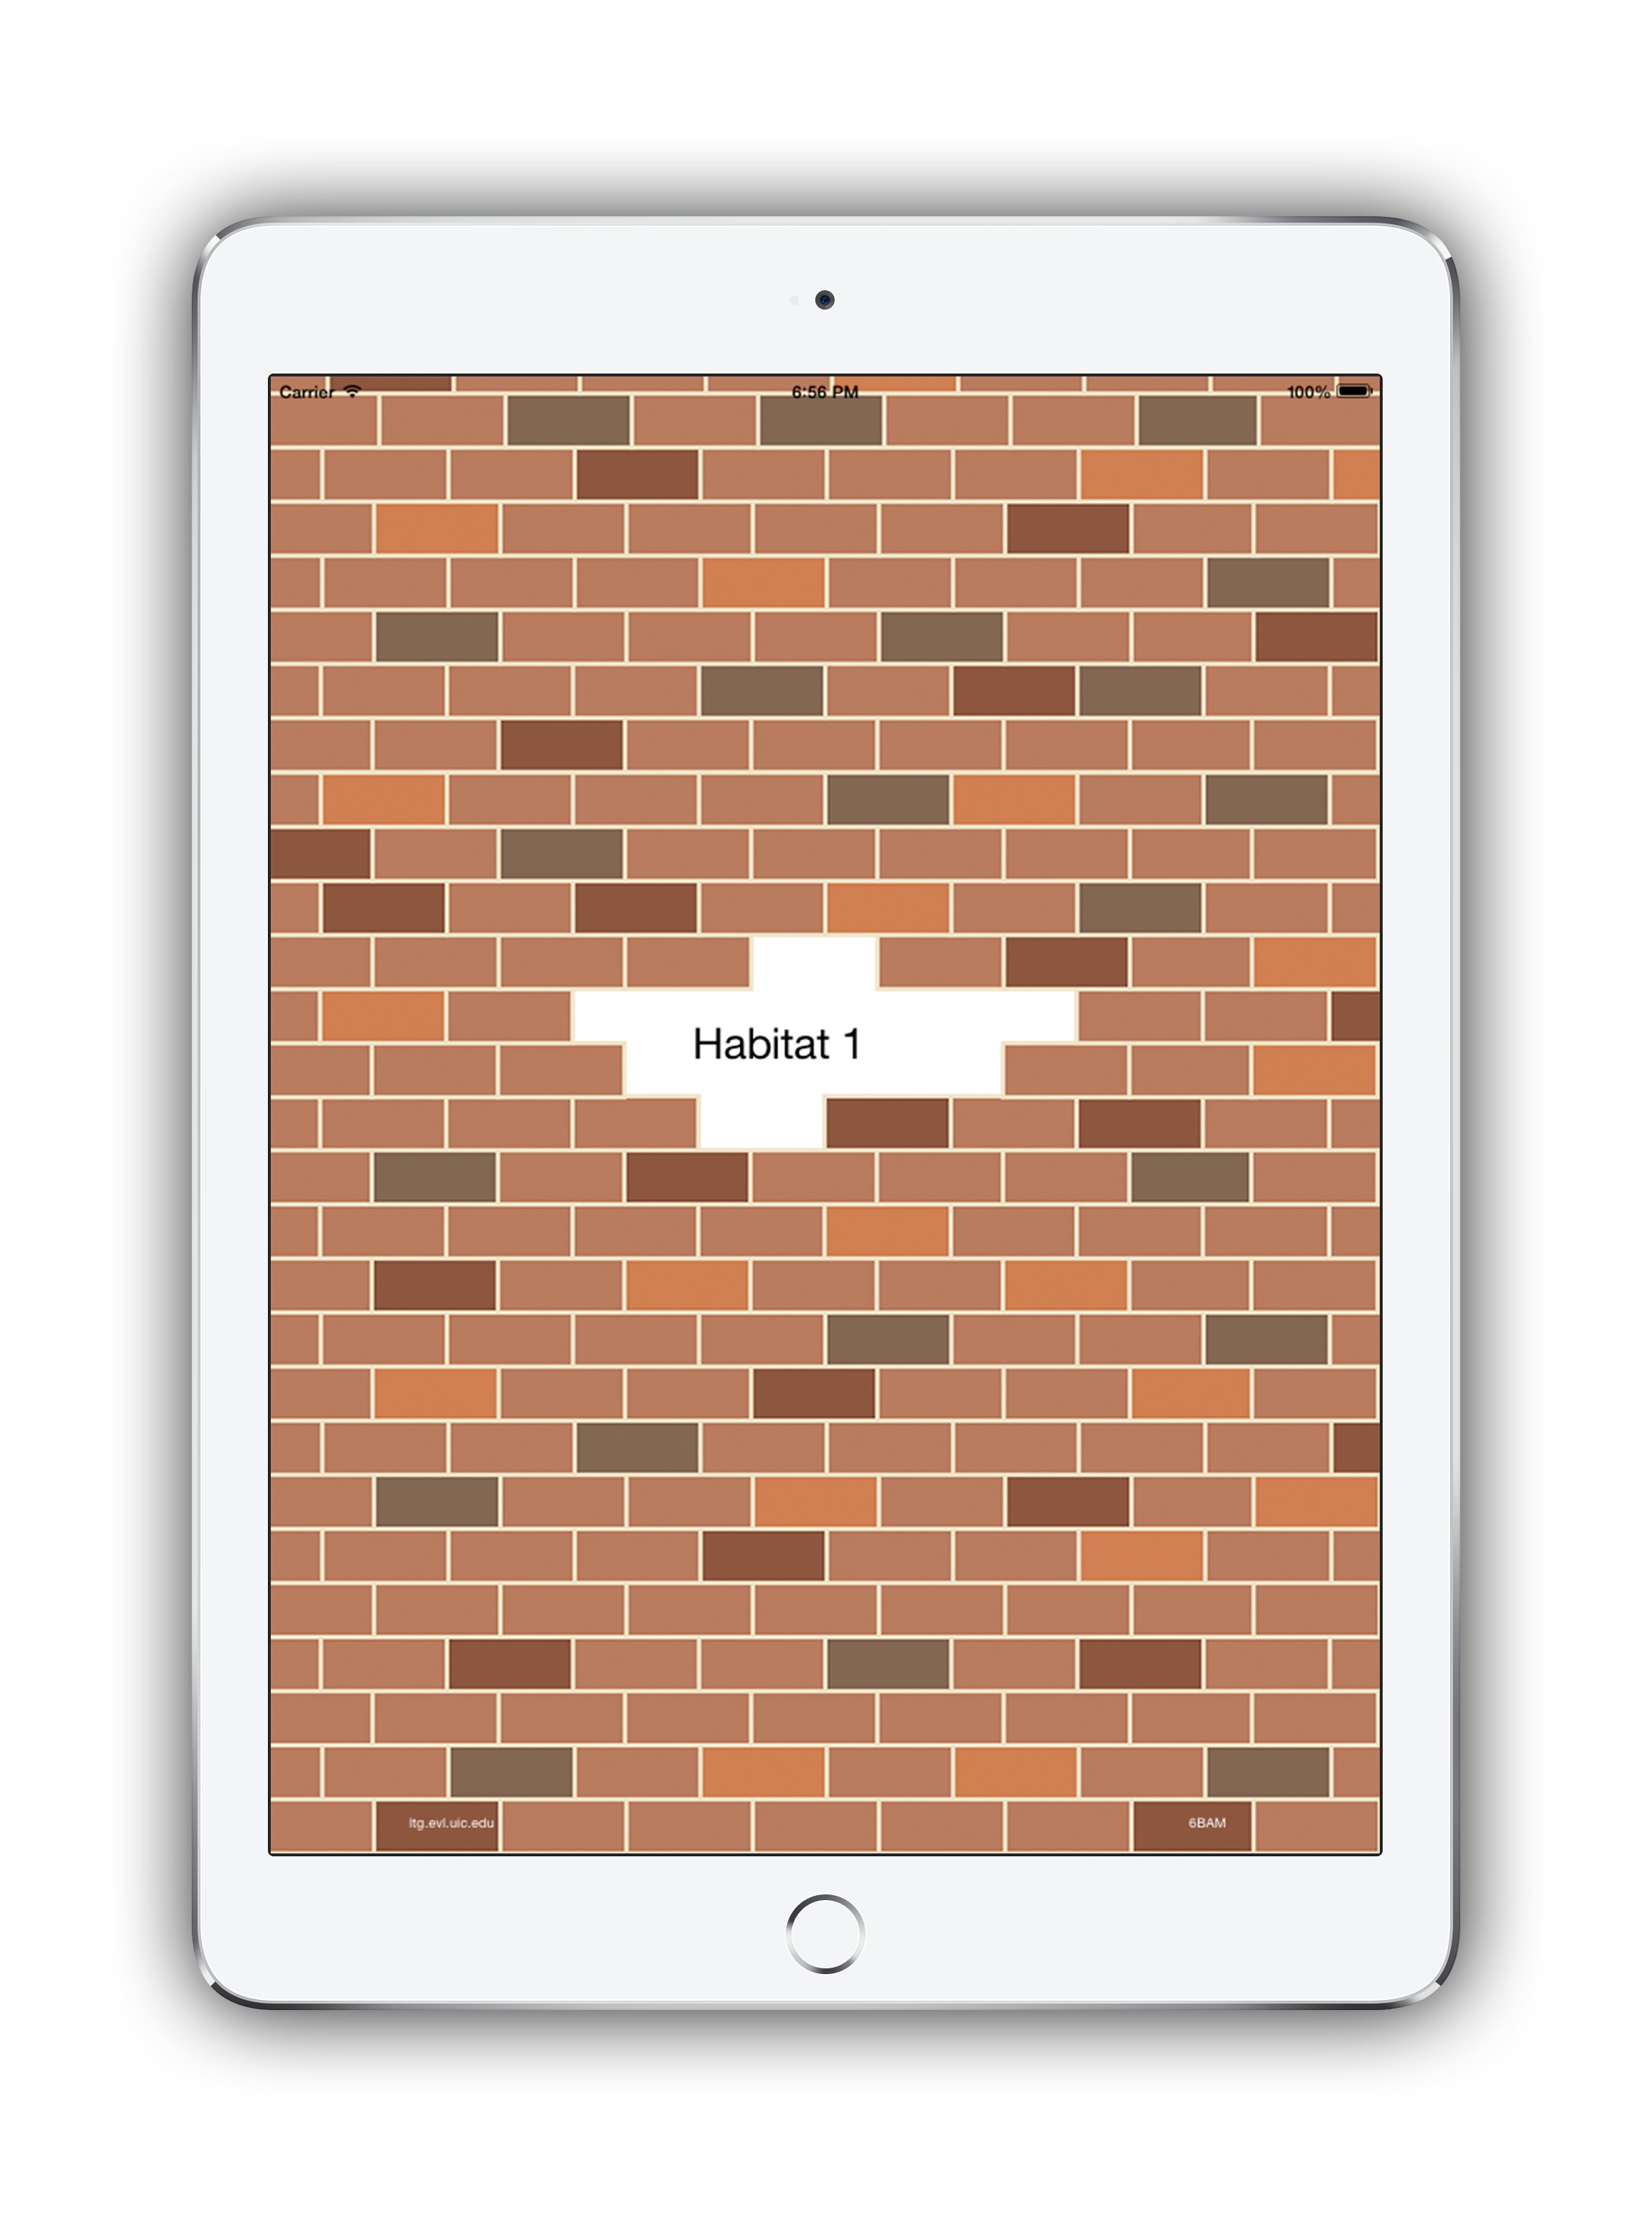
\includegraphics[width=3in]{images/wallcology-ios-sensing.png}
\caption{iOS application while sensing for tangibles}
\label{fig:wallcology_ios_config_sensing}
\end{figure}

\subsection{Simulator bot}
The \textit{Simulator bot} is the component that is in charge to maintain an always running simulation of the ecosystems. There is one instance of this bot for every class. Nutella framework manages when the instances have to start and stop and also the data separation.

This bot has two functions:
\begin{itemize}
\item Update the simulation state every 15 minutes and notify all the components that a change happened.
\item Listen for events coming from \textit{Population Controls} interface and update the state consequently.
\end{itemize}

The simulation state contains the number of creatures of a certain species that are present in every habitat in the present time and also three environmental variables: temperature, pipes level and brick area.

When this bot starts, it requests the last state to the \textit{History bot} and starts the calculations for determining the next state from it. The relations between species (plants, herbivores, predators) are represented using non-linear discrete dynamic systems. This model is stable in certain ranges of temperatures, pipes and bricks area, this will ensure that the effect of every \textit{increase} and \textit{decrease} action will disappear after a certain time and that \textit{insert} and \textit{remove} actions will not generate physically unrealistic behaviors (negative or too many individuals of certain species). At every iteration (every fifteen minutes) a set of equations is used to recalculate the populations living in the ecosystems.

\subsection{History bot}
This bot has the only purpose of listening for state changes and perturbations (on the habitat and on the species) and write them in a persistent object that acts as an hystorical log of everythong happened in the simulation (both the automatic behaviors and the user interactions).

It is possible, in every moment, to query the bot for retrieving the history. \textit{Population History} interface requests this bot for information about the population. It is also used in order to recover \textit{Simulator} bot after a crash or during the normal start-up procedure.

\subsection{RoomCast}
In order to provide classrooms isolation, every component that contains \textit{nutella.lib} needs to know the class identifier (for convention the name of the class was used) and other technical details like the url of the server that hosts the simulation. The bots are entirely managed by \textit{nutella framework} that automatically instantiates all of them providing these parameters automatically behind the scenes when the new run is spawned with \textit{nutella start} command. On the front-end part, where all the interfaces live (inside a browser), it is not possible to automatically provide all the information needed by nutella (run\_id, app\_id, mqtt\_broker\_address). This problem is even more complicated, by the fact that every interface needs also other information (e.g. the habitat that it must be displayed on that specific computer of the class). By design all those information is concentrated in only one point: the url of the interface. This choice allow to debug the application simply opening an url in the browser. The drawback is that every time students need the tool a very long url must be manually inserted. This problem could be solved with browser bookmarks, but with a very bad user experience while passing form one interface to another. It also had required a lot of manual work because every link must be manually inserted (not a very scalable solution).

In order to simplify the setup of the ecosystems in the three classes it was created a sophisticated environment for providing all the tools in only one web page and allow the students to easily switch from one interface to another without changing browser window, this tool is called RoomCast. In this section I describe the RoomCast parts that were useful during the study.

\begin{figure}
\centering
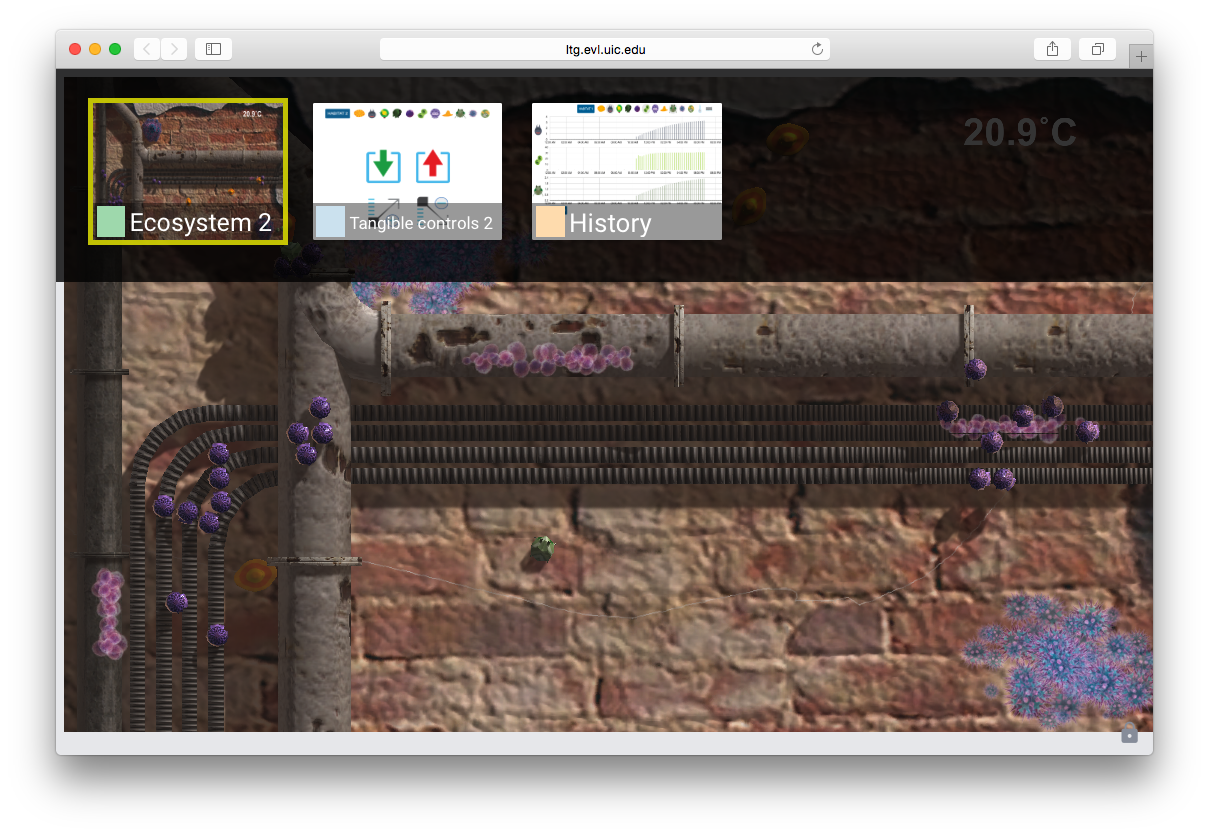
\includegraphics[width=4.5in]{images/room-cast-menu.png}
\caption{RoomCast menu for selecting the interface}
\label{fig:roomcast_menu}
\end{figure}

RoomCast is an interface that wraps all the other nutella interfaces and has the following functionalities:
\begin{itemize}
\item Provides a menu for switching from the current interface to another (\ref{fig:roomcast_menu}).
\item Provides an authentication method that allow to select the classroom and the ecosystem number (\ref{fig:roomcast_classroom}).
\item Provides a teacher interface that is used for controlling which tools are available (\ref{fig:roomcast_role}).
\end{itemize}
The authentication function is important for allowing only the right functions on the specified computer. At the beginning of every lessons, the browser starts automatically on every computer in full-screen mode and the only action required by the teacher is clicking on the name of the current class and current habitat. From that moment on all the interfaces are automatically personalized (the parameters are passed to the interfaces and the url is hidden from the user).

In order to select an interface, the students can click on the pink button present in the top left corner (\ref{fig:population_controls_locked}) of the screen (it can be also moved) in order to show the menu with all the enabled interfaces. In order to control software anomalies in the interfaces a reload button is inserted (blue button in \ref{fig:population_controls_locked}), the button reloads only the current interface without requiring all the others to update. It can also be activated remotely without the user intervention.

\begin{figure}
\centering
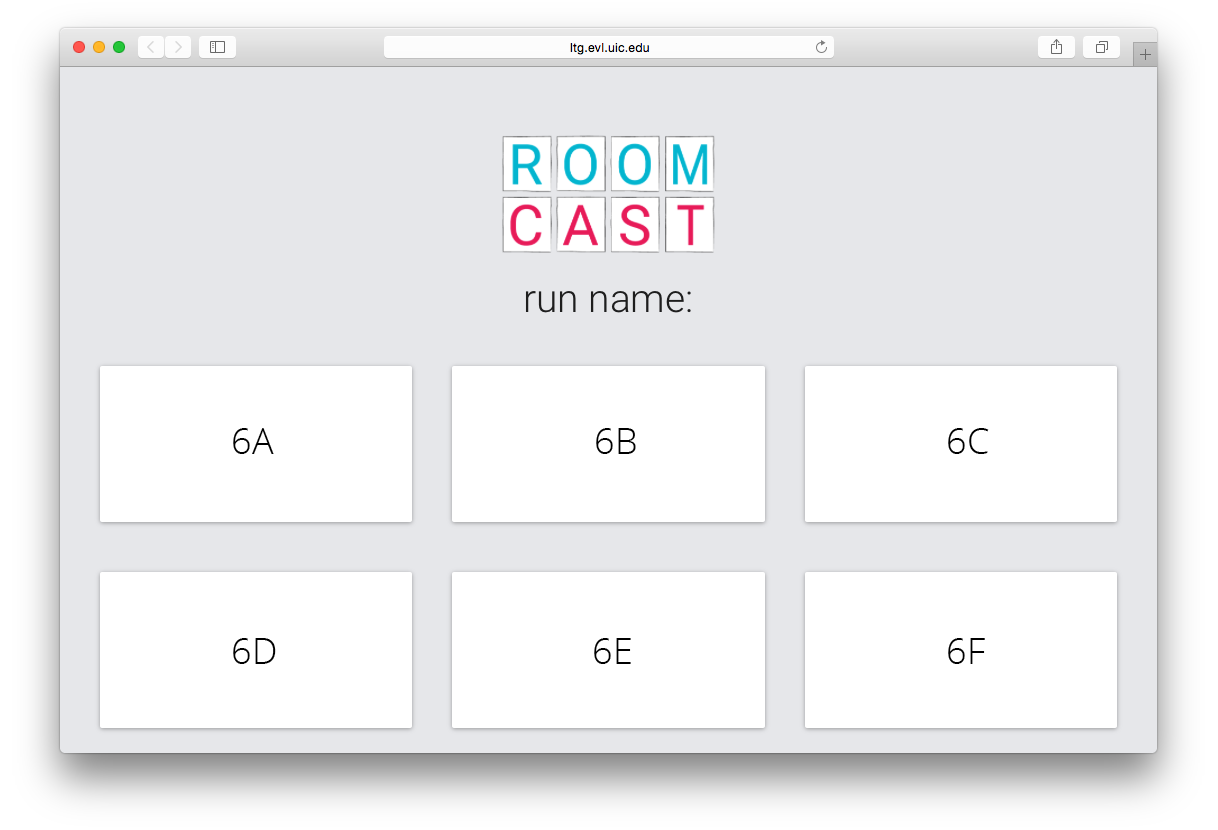
\includegraphics[width=4.5in]{images/room-cast-classroom-selection.png}
\caption{RoomCast interface for the selection of the class}
\label{fig:roomcast_classroom}
\end{figure}

\begin{figure}
\centering
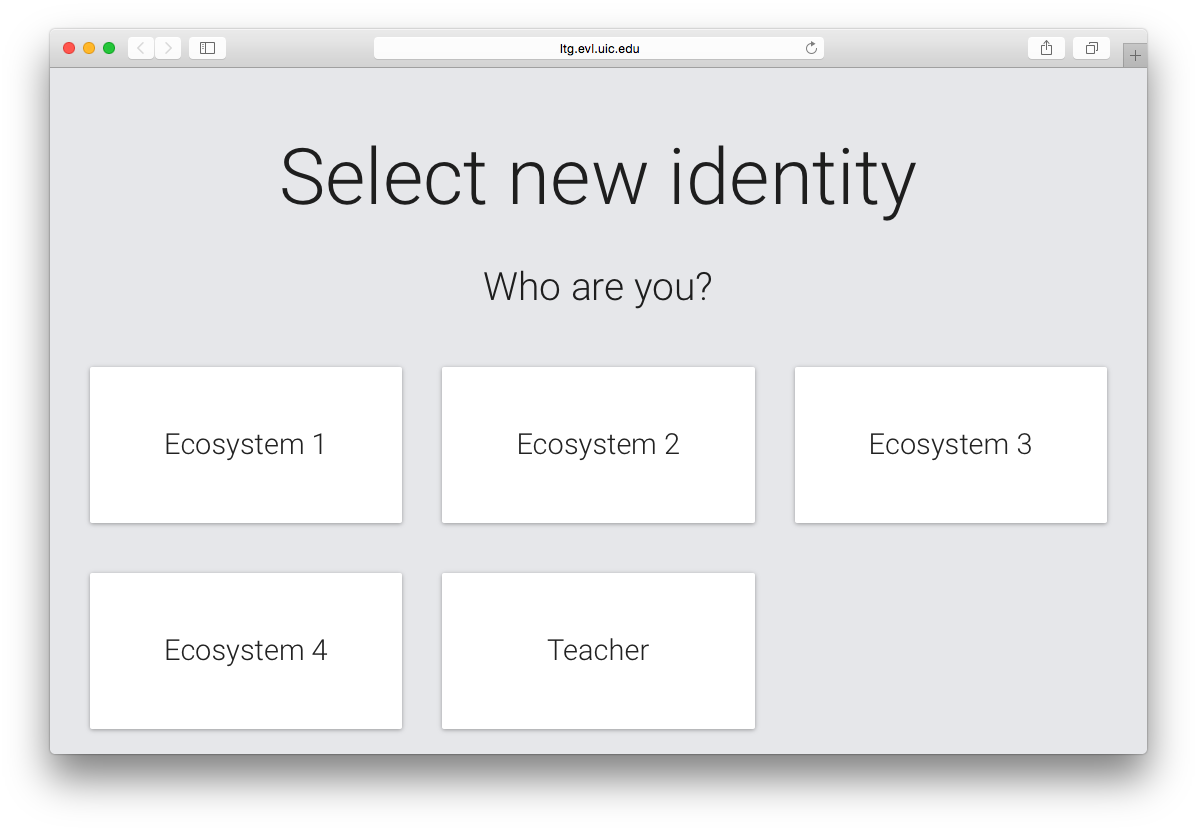
\includegraphics[width=4.5in]{images/room-cast-habitat-selection.png}
\caption{RoomCast interface for the selection of the role}
\label{fig:roomcast_role}
\end{figure}

\section{Research method and data sources}
For answering the research questions, I decided to study children behavior during the class activities that involve the usage of beacons: those activities are called \textit{perturbations} because they modify (\textit{perturb}) the habitat in a number of different ways through the \textit{population control} interface (already explained at the beginning of this section).

The experiment was conducted on three classes of primary school and with a total of 48 children. Two physical room were used: one spacious science laboratory with four desktop computers, positioned on the four walls and one classroom in which four laptops were positioned before the beginning of every lesson. The metaphor used in this study is that every computer is an habitat, a group of four students is assigned to every habitat.

Three different data sources were used for collecting evidence:
\begin{itemize}
    \item Video recordings, simultaneously from four cameras:
    \begin{itemize}
        \item A fixed camera on the ceiling pointing at habitat 1.
        \item A fixed camera on a shelf capturing the entire room.
        \item A moving camera on a tripod, always filming the current activity and the center of attention of the class.
        \item A smartphone camera operated by a researcher, activated when discussion happen inside a student group
    \end{itemize}
    \item Questionnaire for children with 5 questions asking different aspects of the interaction with tangibles
    \item Software interface action logging
\end{itemize}

The two fixed cameras were used only in the science laboratory because it was the only place where the computer remained in the same position all the time, in the other classroom the laptops moved every lesson and also during the activities. 

A major challenge that video recordings presented was the collection of evidence of discourses between students about the scientific topic. The task was difficult because they happened in different areas of the class simultaneously between 16 students and it was not easy to predict the best place to record with the moving cameras. The method applied was to continuously film one habitat with a fixed camera recording everything happened there. Use a shelf mounted fixed camera without audio for recording all student-to-student interactions for distinguishing when they happen between students of the same group or between students of different groups. Use the smartphone camera and a tripod mounted camera for capturing single discourses taking place near the researcher and moving rapidly from one group to the others in order to capture the maximum number of conversations.

The questionnaire was assigned to the students to complete after they tried both the web interface and the tangibles in order to make a perturbation. The web interface and the tangible interface show exactly the same elements on the screen, with the only difference that when the tangibles were enabled students could not use the mouse for interacting (except for confirming the action).

The last data collection method is based on writing a log (on the server using nutella capabilities) that records every time which interface is used for doing the perturbation (tangibles or web interface), on which habitat is done and who does it (the teacher or the students). This method is not really useful because at the beginning of each lecture the teacher forced the students to use one interface or the other, but is a confirmation for us that the system is working and provides information on what really happened. The teacher interface was entirely operated by me in order to change habitats conditions. Sometimes certain groups discussed longer than others and didn't have time to do the perturbation during the lecture. The teacher interface was also used in order to change the amount of pipes present in some ecosystems that is an action that students are not allowed to do.

\subsection{Tangibles creation and RoomPlaces integration}
Tangibles are the interface that children have the opportunity to use and that are subject of this study. For this reason a huge amount of time was invested in order to design and build solid, pleasant and funny creatures that have the possibility to became valuable practice-linked resources and possibly cultural artifact \cite{horn:role}. During the design phase three elements were kept into account:
\begin{itemize}
\item Possibility of embedding an iBeacon sensor inside them
\item High fidelity of the final result with the 3D model present in the animation
\item High quality of the final result in term of robustness and impact resistance 
\end{itemize}

The design phase is divided in two parts: the design of the iBeacon container and the design of the creatures. During both the phases Maya 3D modeling software was employed. The first phase required to measure the beacon size and to create a cavity inside a base that was used to contain the Bluetooth LE emitter. The second phase took more time because it required to model all the creatures, it was done only once for both creating the simulation and the tangibles.

The 3D models were created with a 3D printer. The chosen material was tested against Bluetooth signal attenuation. They were painted in order to replicate the exact same texture of the creatures in the simulation and glued with the base where the iBeacon was inserted. The final result is shown in \ref{fig:tangibles}. For the other tangibles: 4 species, 4 actions and 4 keys the graphic icons were printed, laminated and glued on the beacon base.

\begin{figure}
\centering
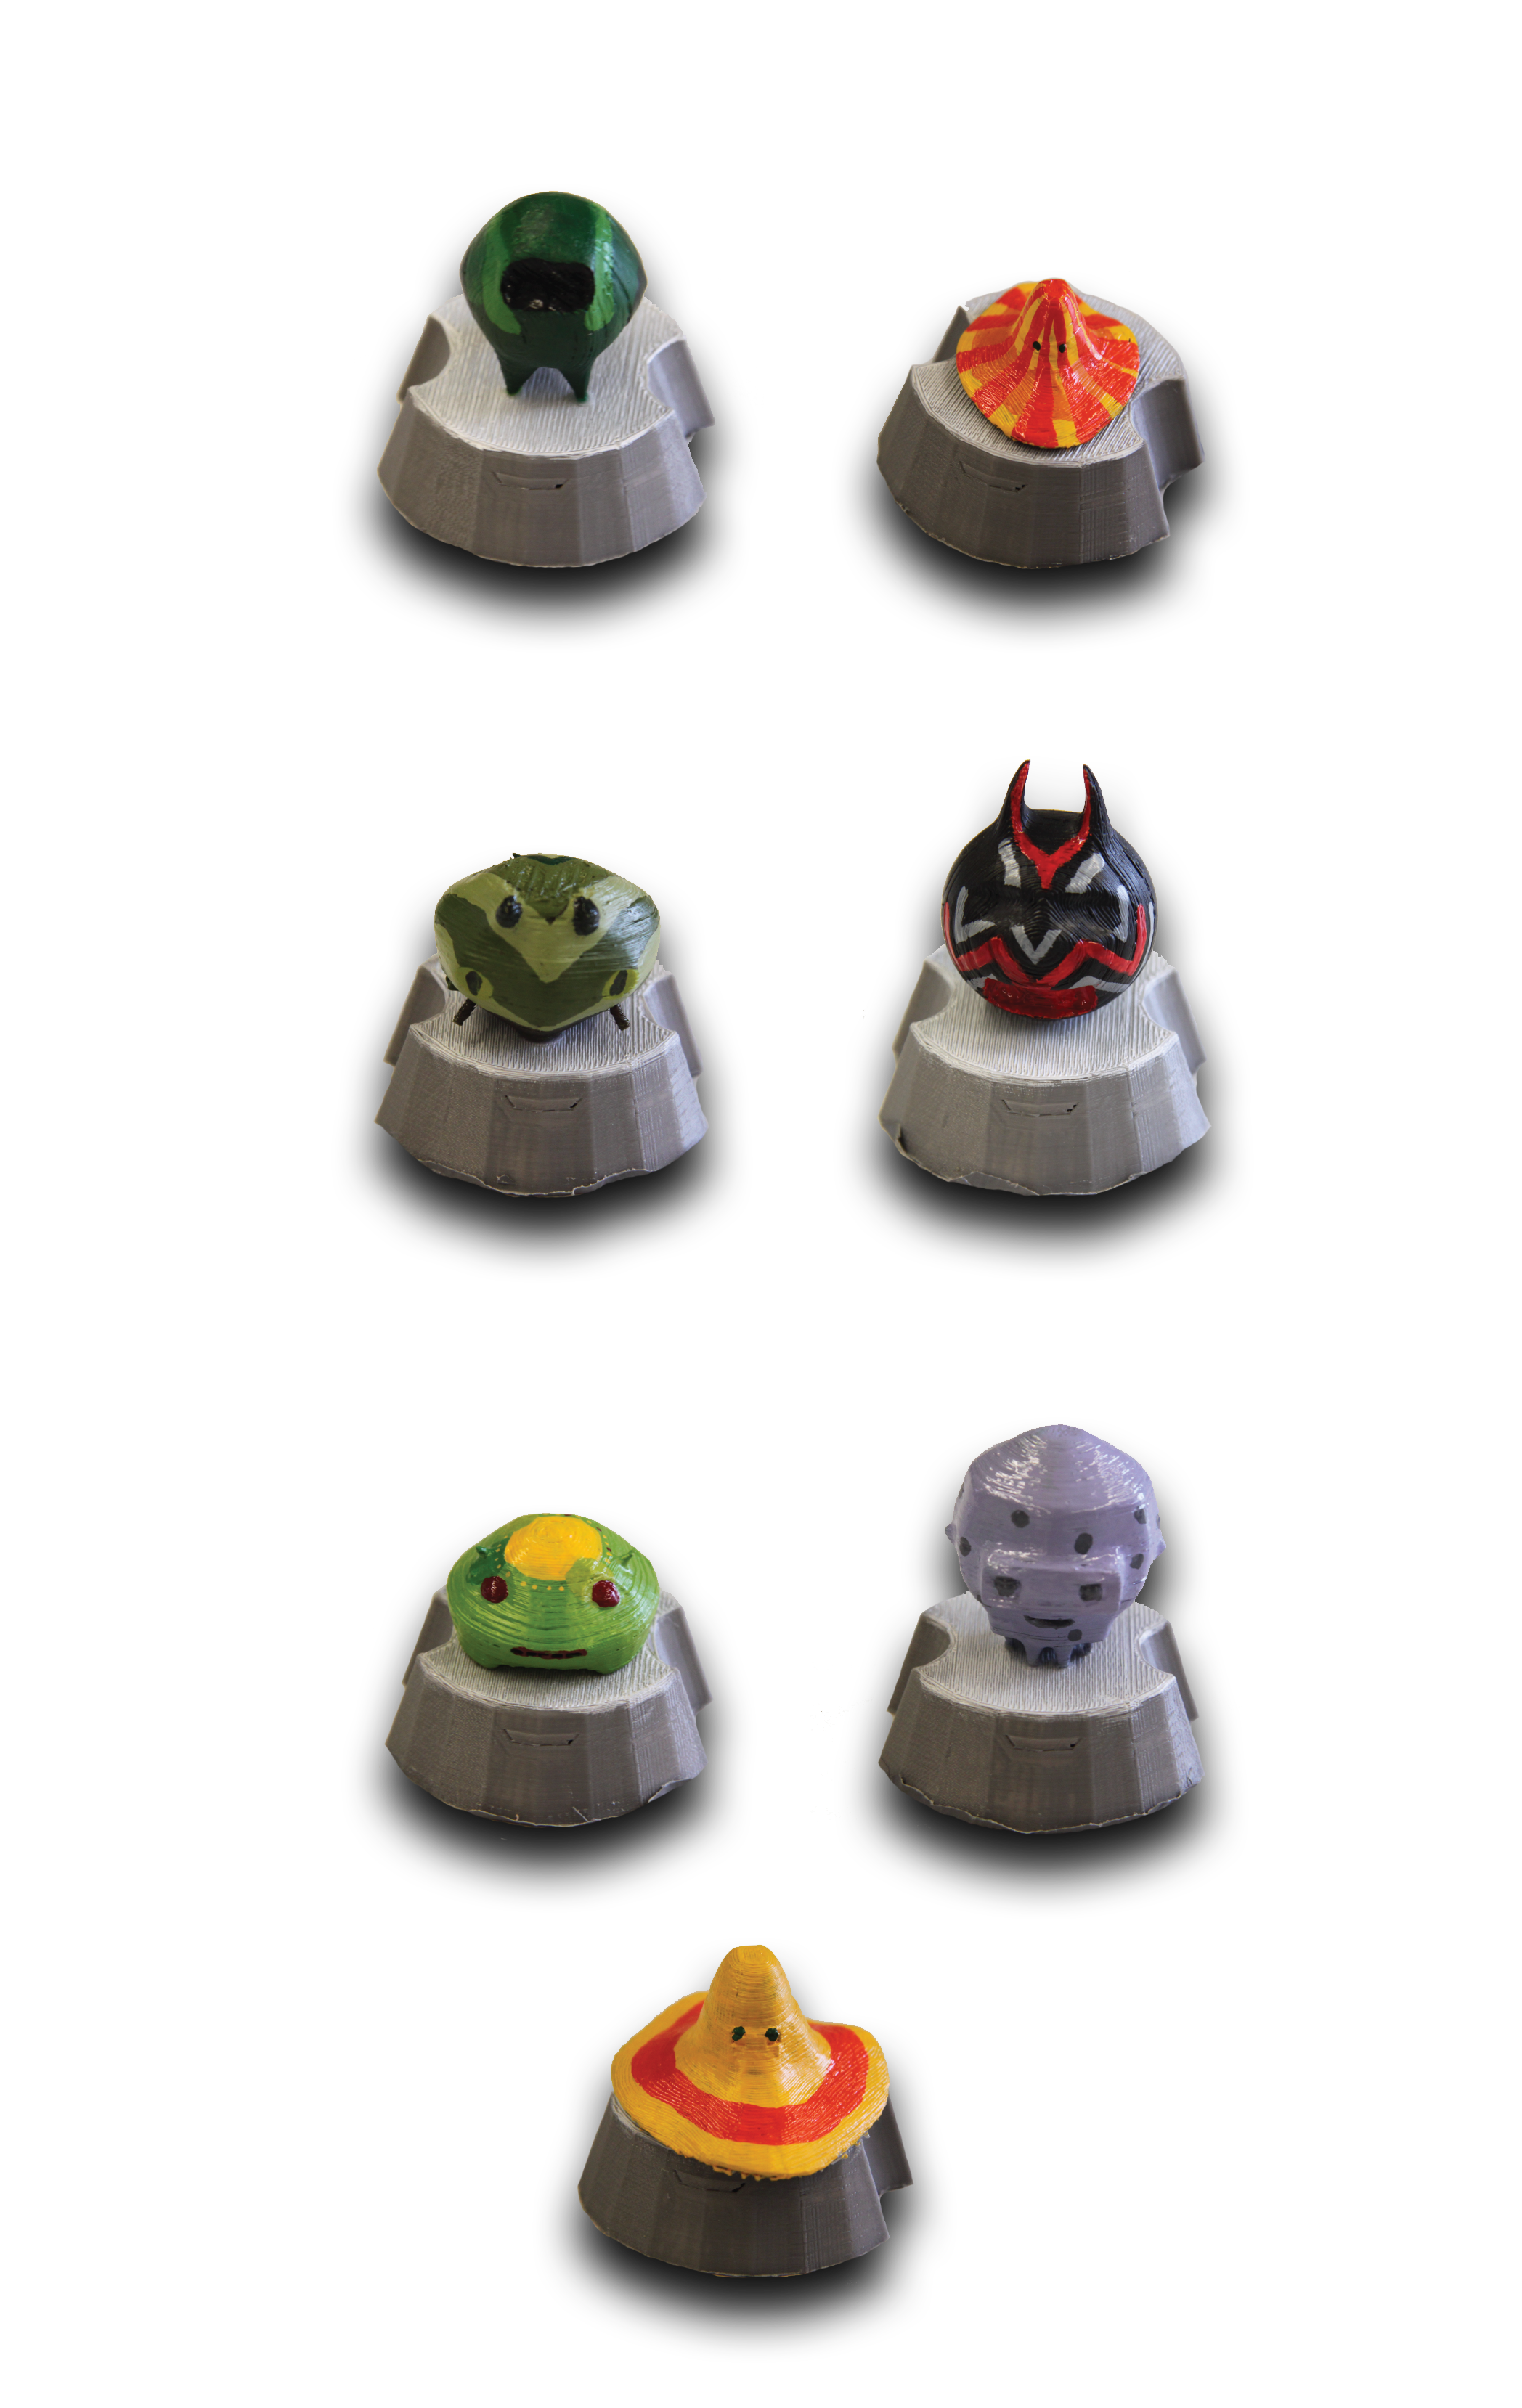
\includegraphics[width=5in]{images/tangibles.png}
\caption{Seven creature tangibles printed in 3D}
\label{fig:tangibles}
\end{figure}

Every tangible contains exactly one beacon that was previously registered in the system using the \textit{Beacon Cloud} interface and inserted in every class using \textit{Classroom Layout} interface. In order to simplify the substitution of the beacons (inside tangibles), in case of hardware failure, the \textit{resource identifier} of the beacon is  printed on the bottom of the base.

\section{Results}
In this section I report the results of the exploratory study and I give answers to the research questions supported by evidence that I collected using the data sources.

\subsection{Tangibles improve children enjoyment}
In this story, I support with evidence my expectation that tangibles can improve the quality of the lectures, engaging students in funny activities, stimulating their curiosity and letting them focus better on the topic keeping high the motivation.

During the study, in order to develop a personal connection with the creatures, teachers let students chose the names (reported in \ref{tab:species_names}). Every class chose different names for the species and many students had the opportunity to personally assign the names. There are evidence in the video that show how children are excited when they play with the creature they named.

\begin{table}
\centering
\caption{NAMES ASSIGNED BY STUDENTS TO CREATURES}
\begin{tabular}{ | c | c | c | c | c | }
\hline
Species   & Icon & Name 6A & Name 6B & Name 6C \\
\hline
Species 0  & 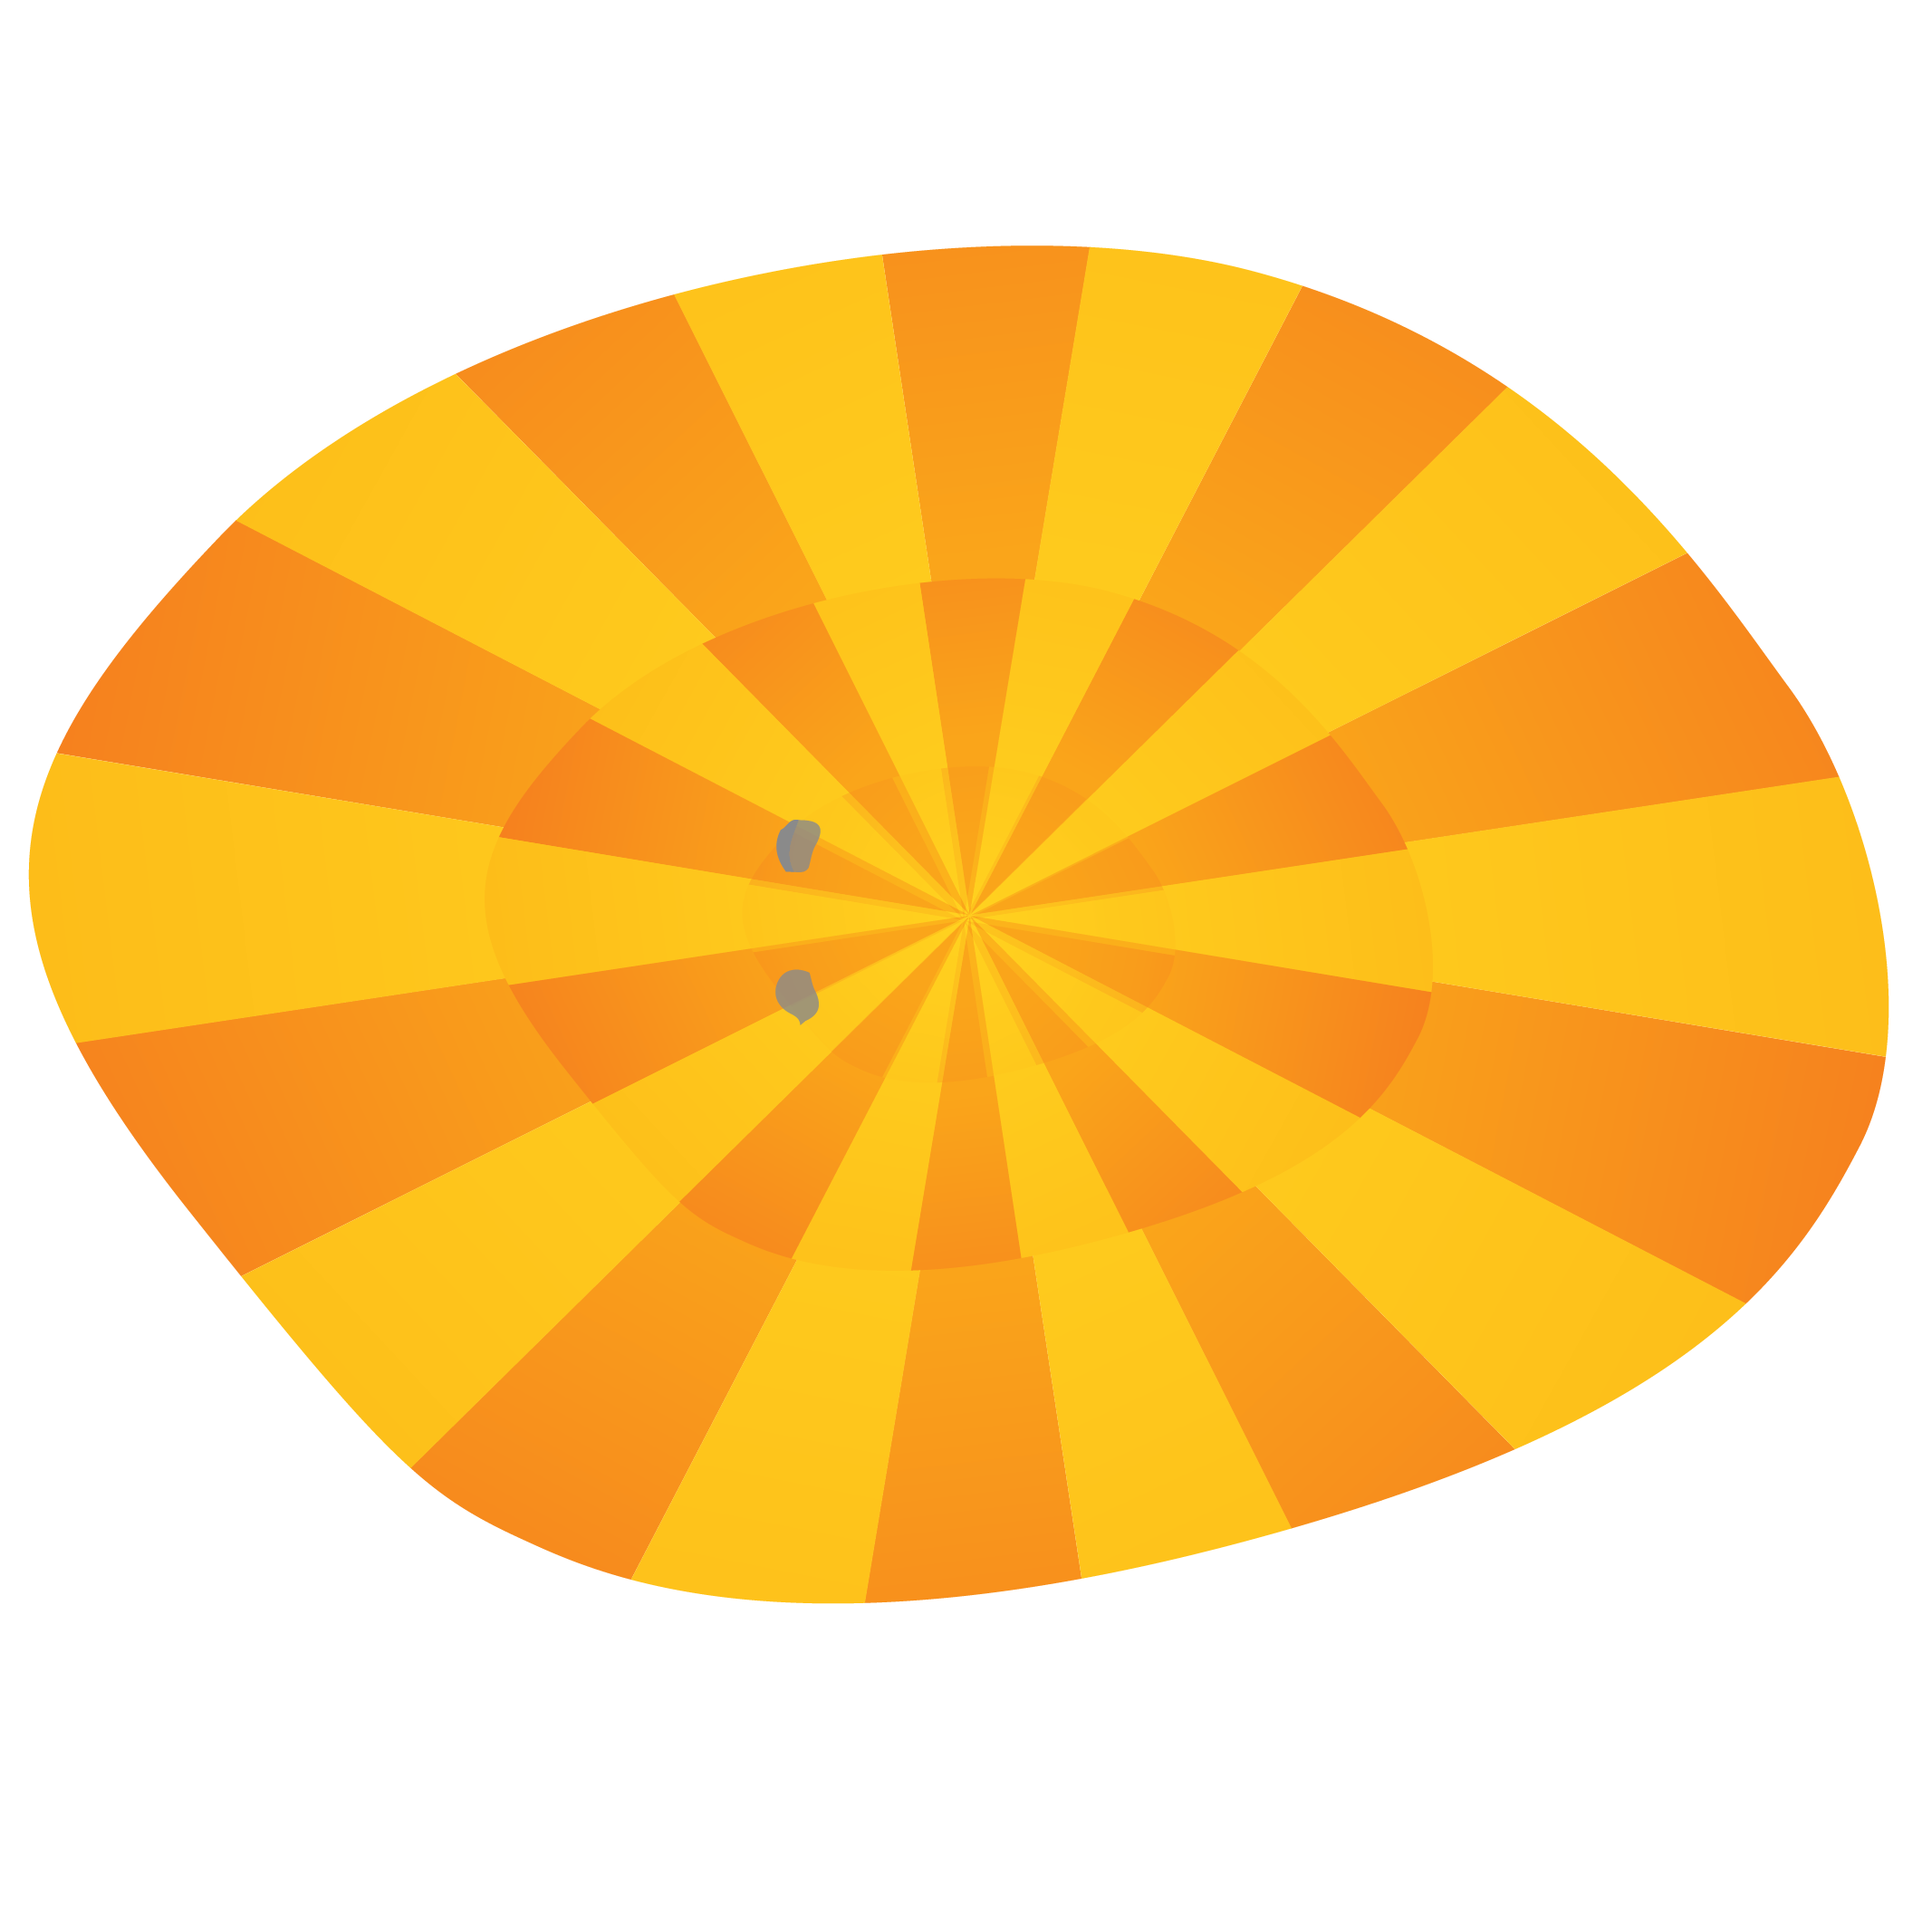
\includegraphics[valign=m,scale=0.1]{images/species_00.png} & Here Comes the Sun & \#imgetendizey & Baby Egg \\ 
Species 1  & 
\includegraphics[valign=m,scale=0.1]{images/species_01.png} & Vampire & Terminator & Batman \\ 
Species 2  & 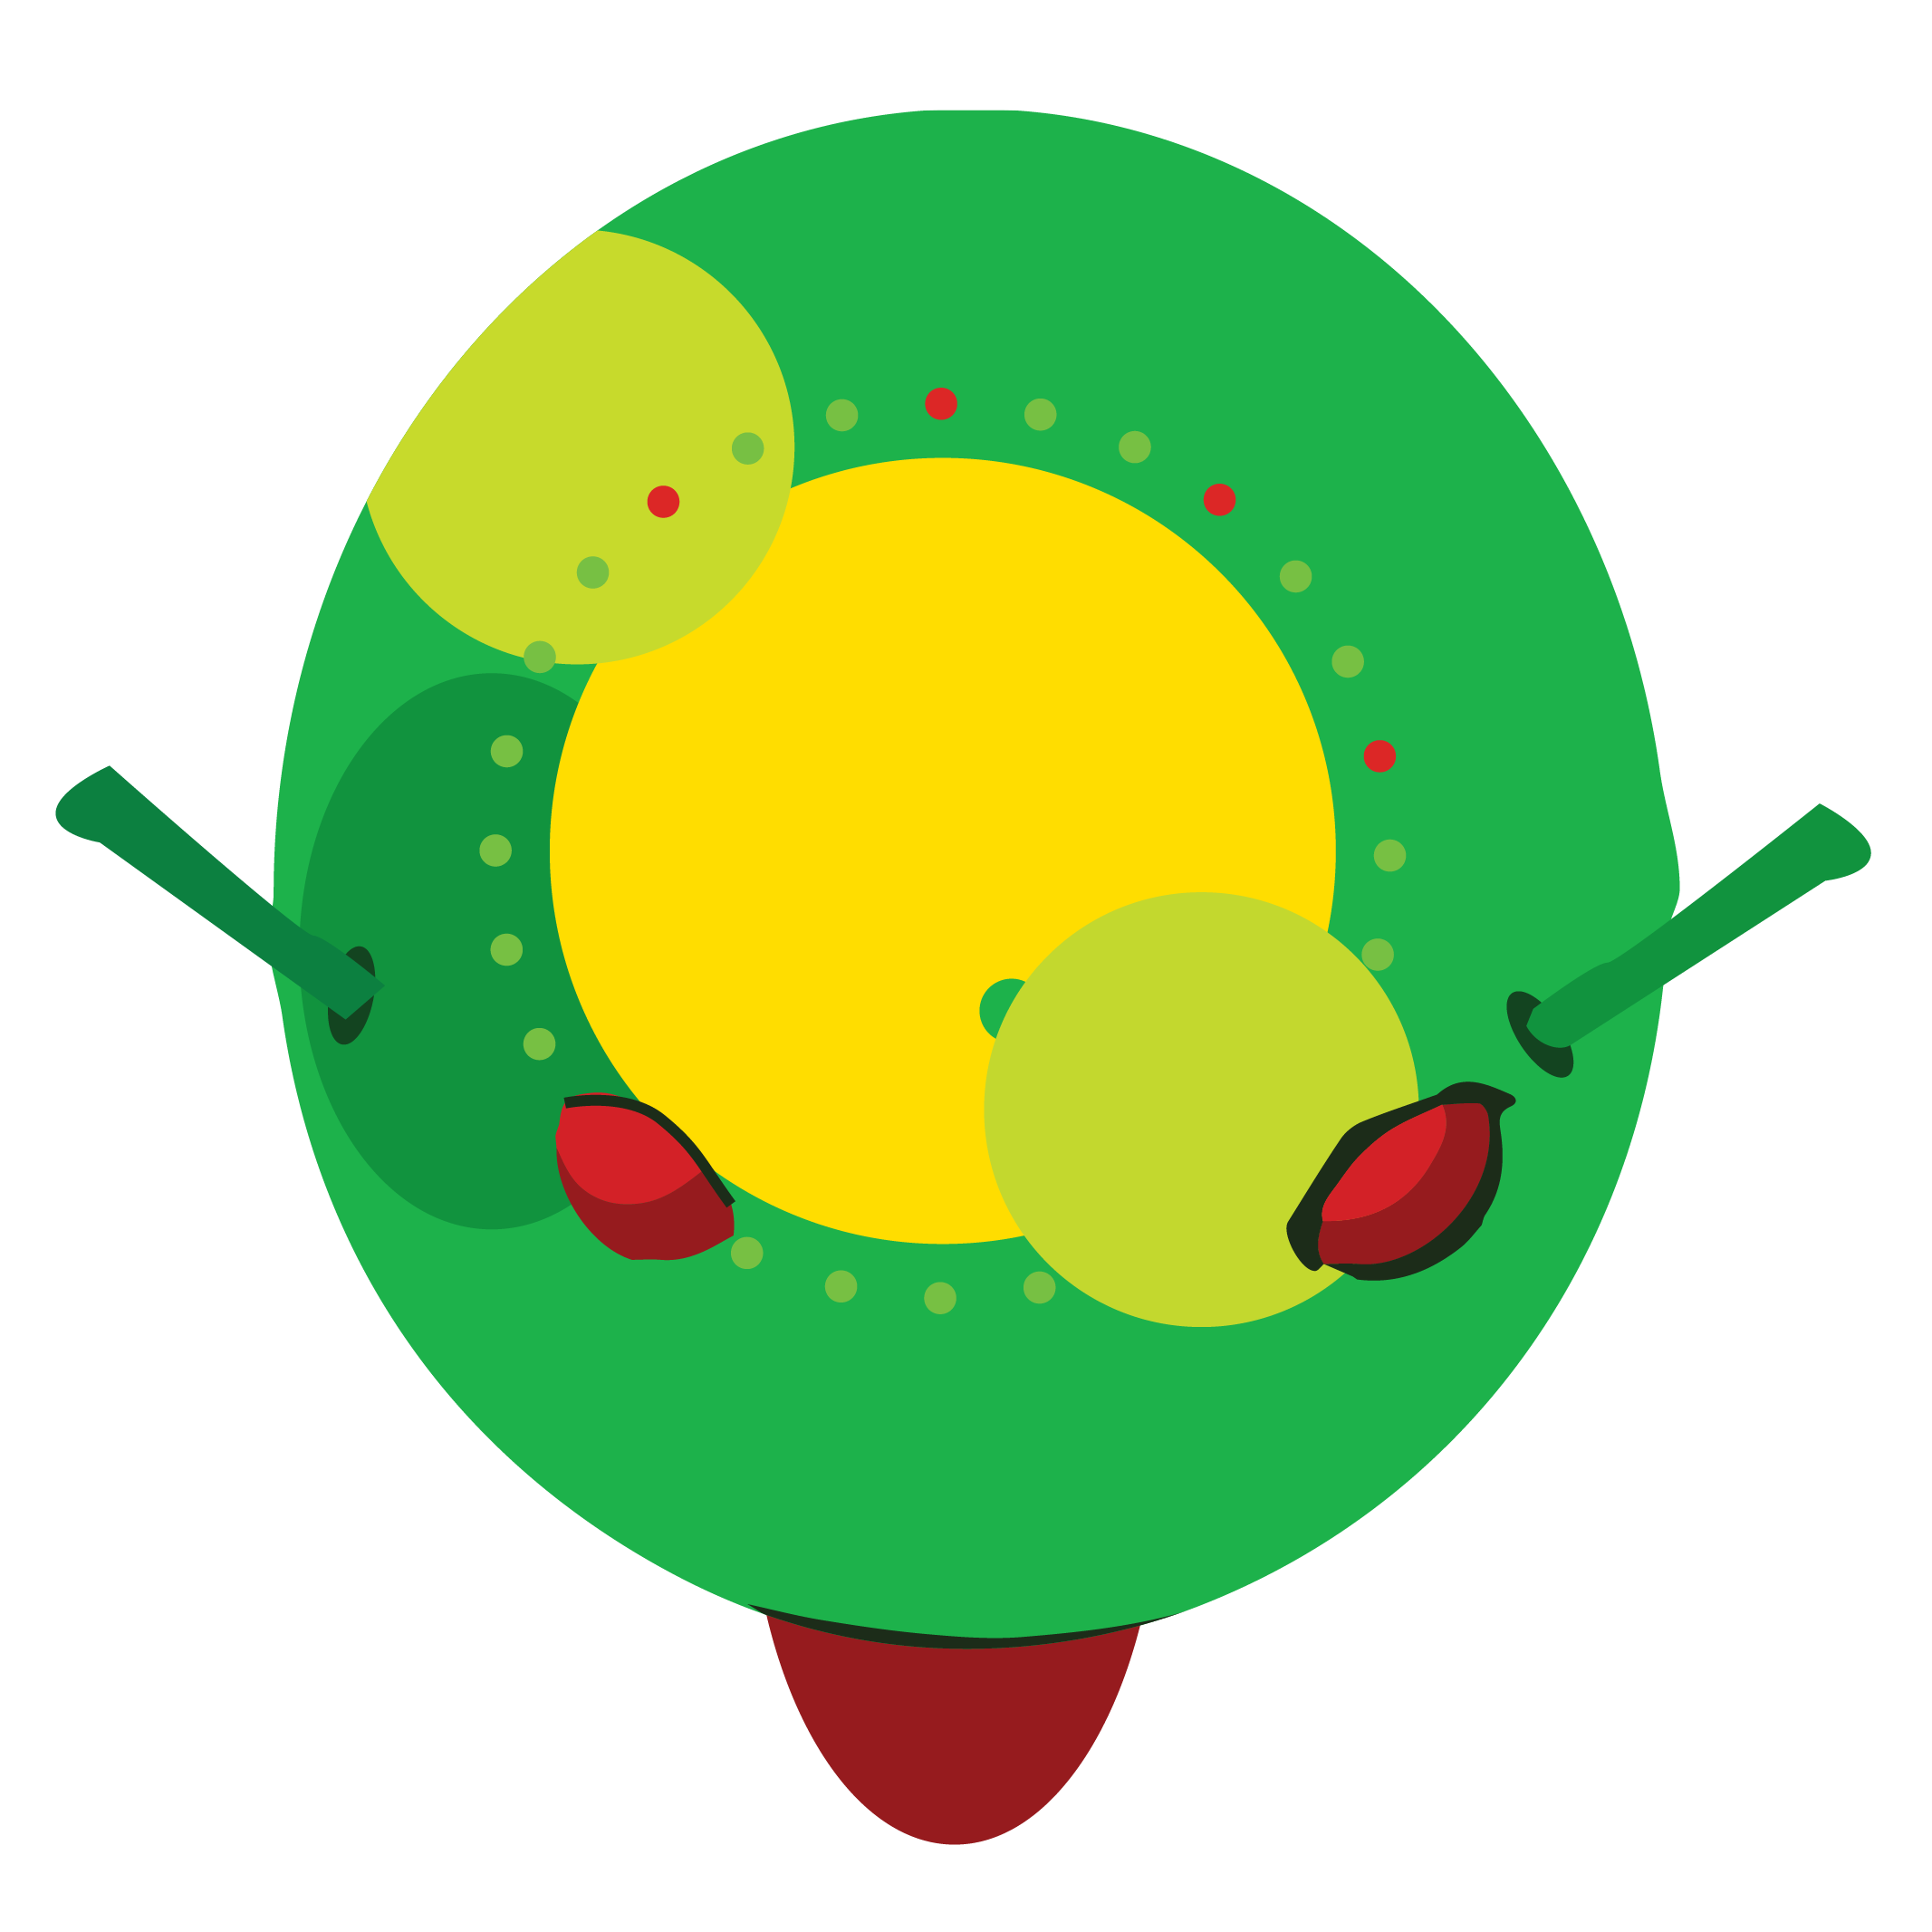
\includegraphics[valign=m,scale=0.1]{images/species_02.png} & Little Tongue & Bol & Toad \\ 
Species 3  & 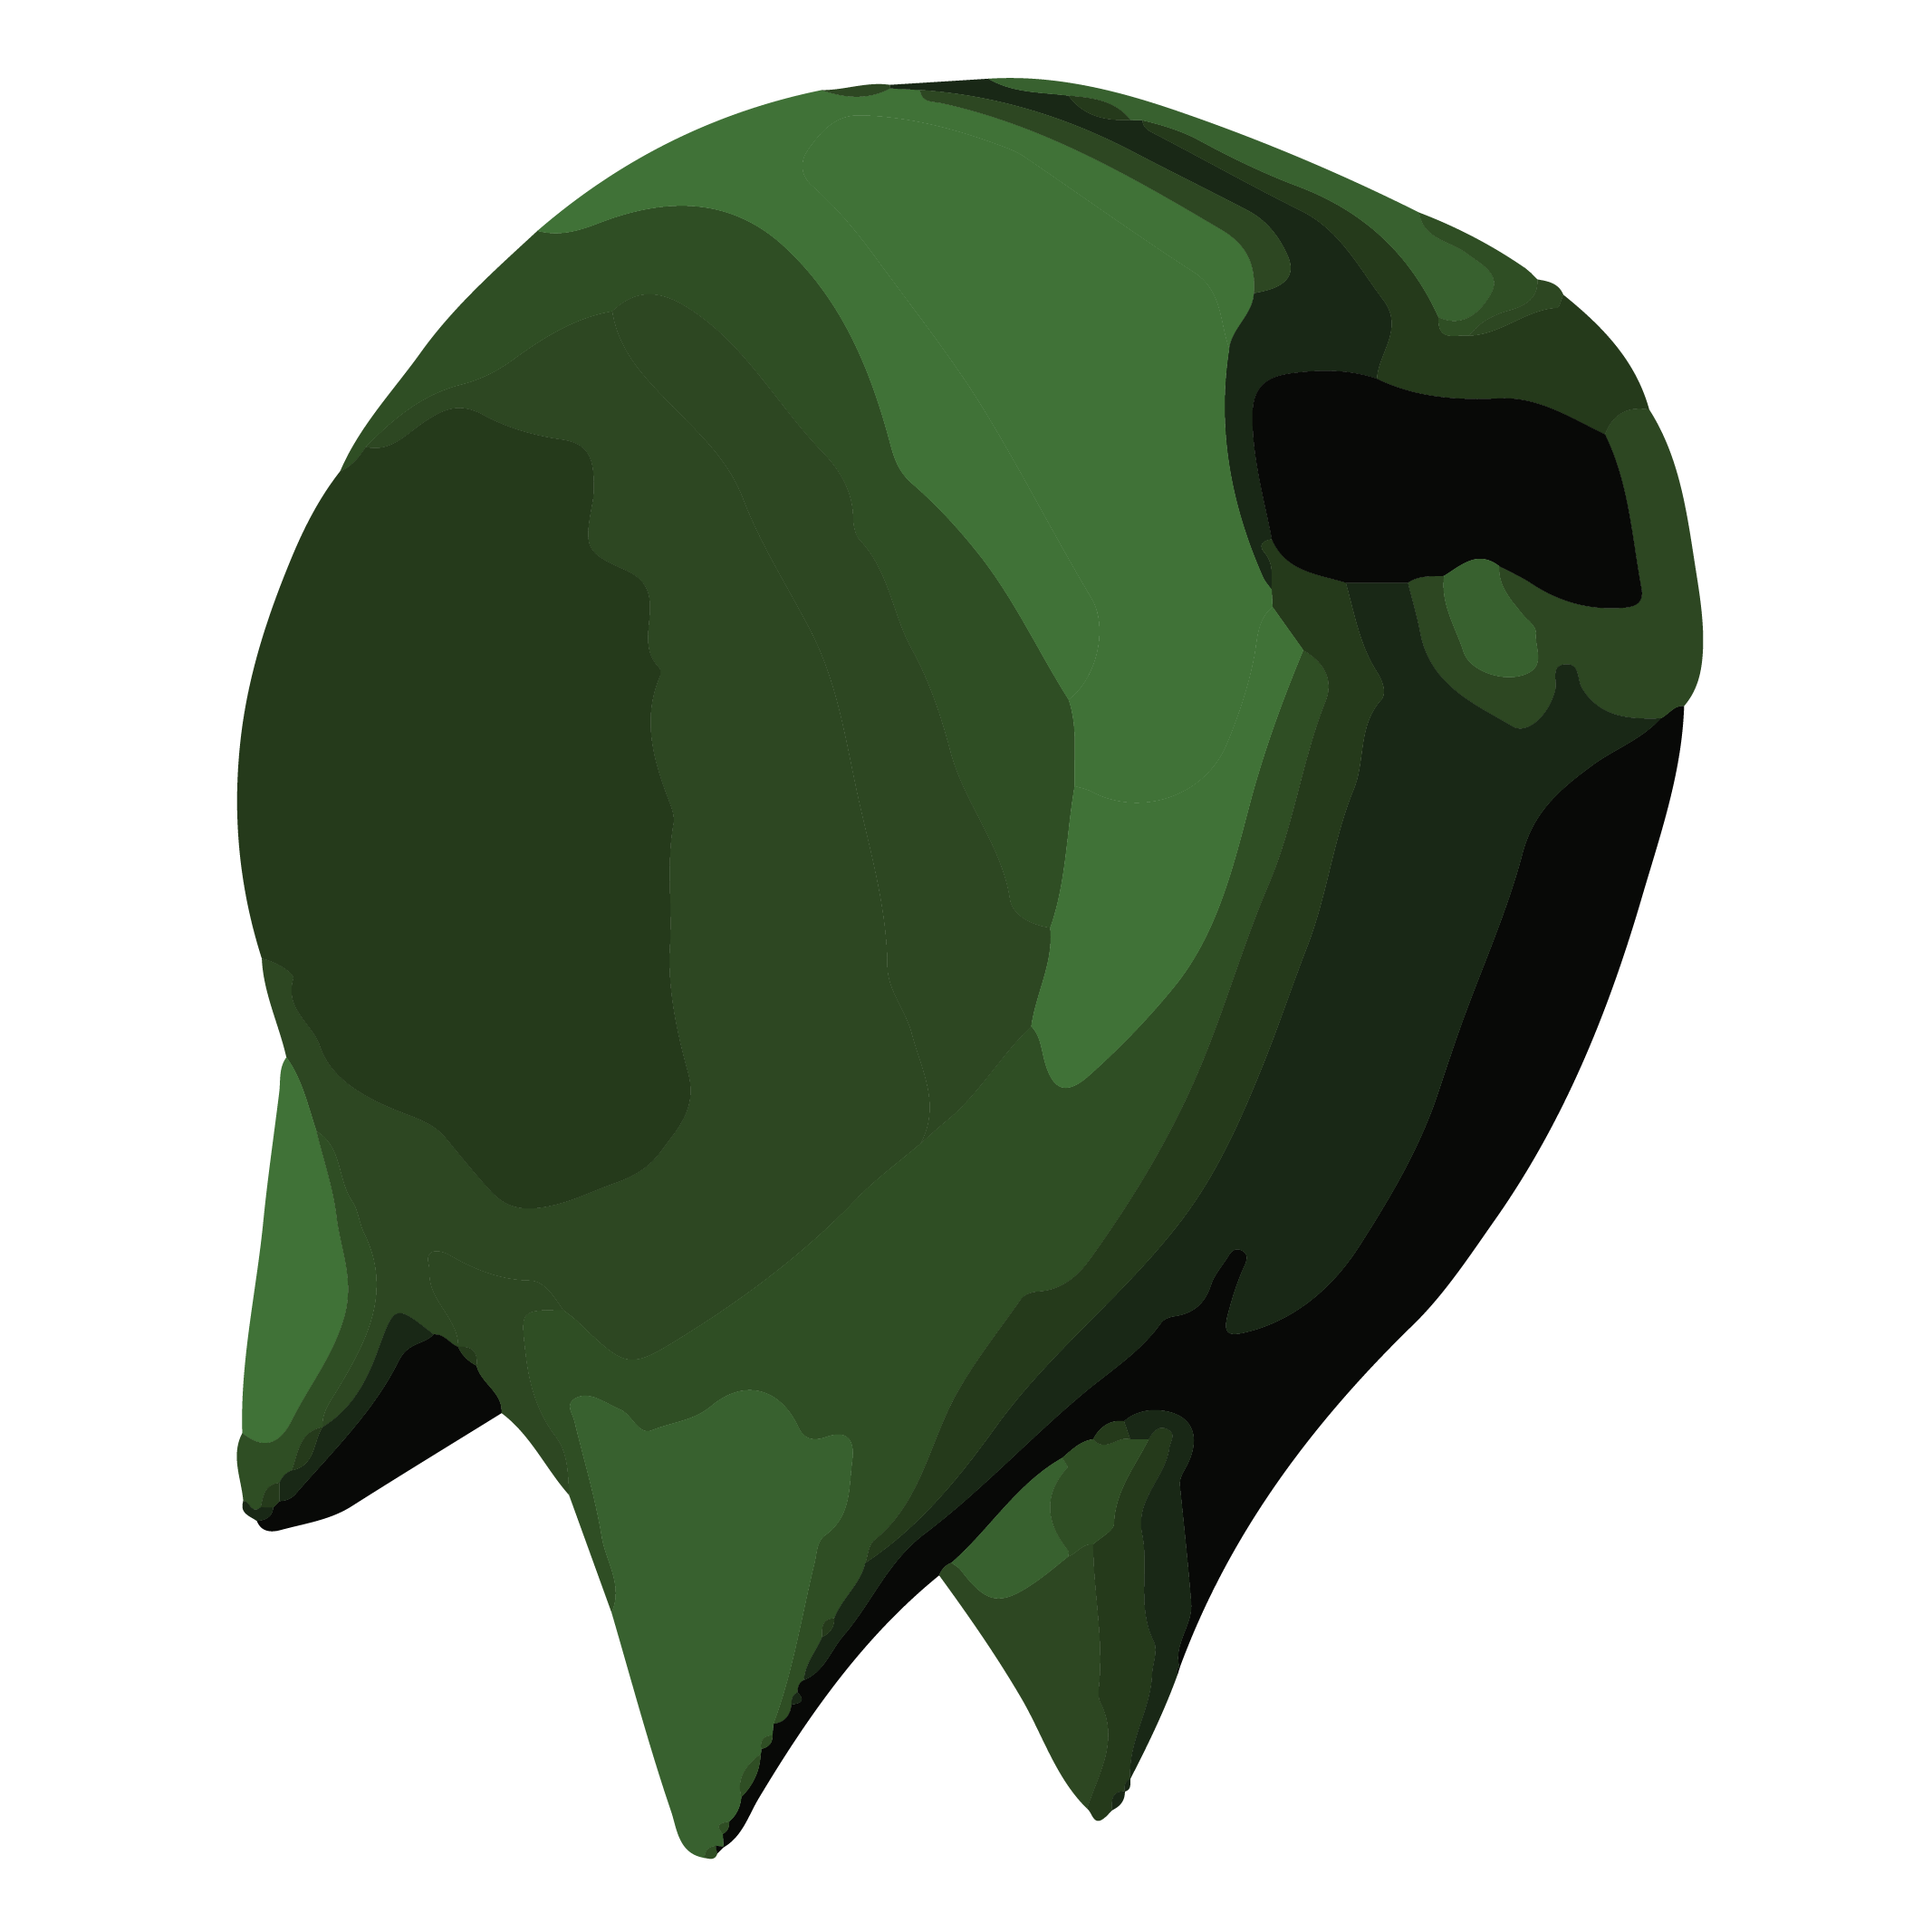
\includegraphics[valign=m,scale=0.1]{images/species_03.png} & Grenngranate & Darock & Broc \\ 
Species 4  & 
\includegraphics[valign=m,scale=0.1]{images/species_04.png} & Purpleberry & Purple Cabbage & Sorbet \\ 
Species 5  & 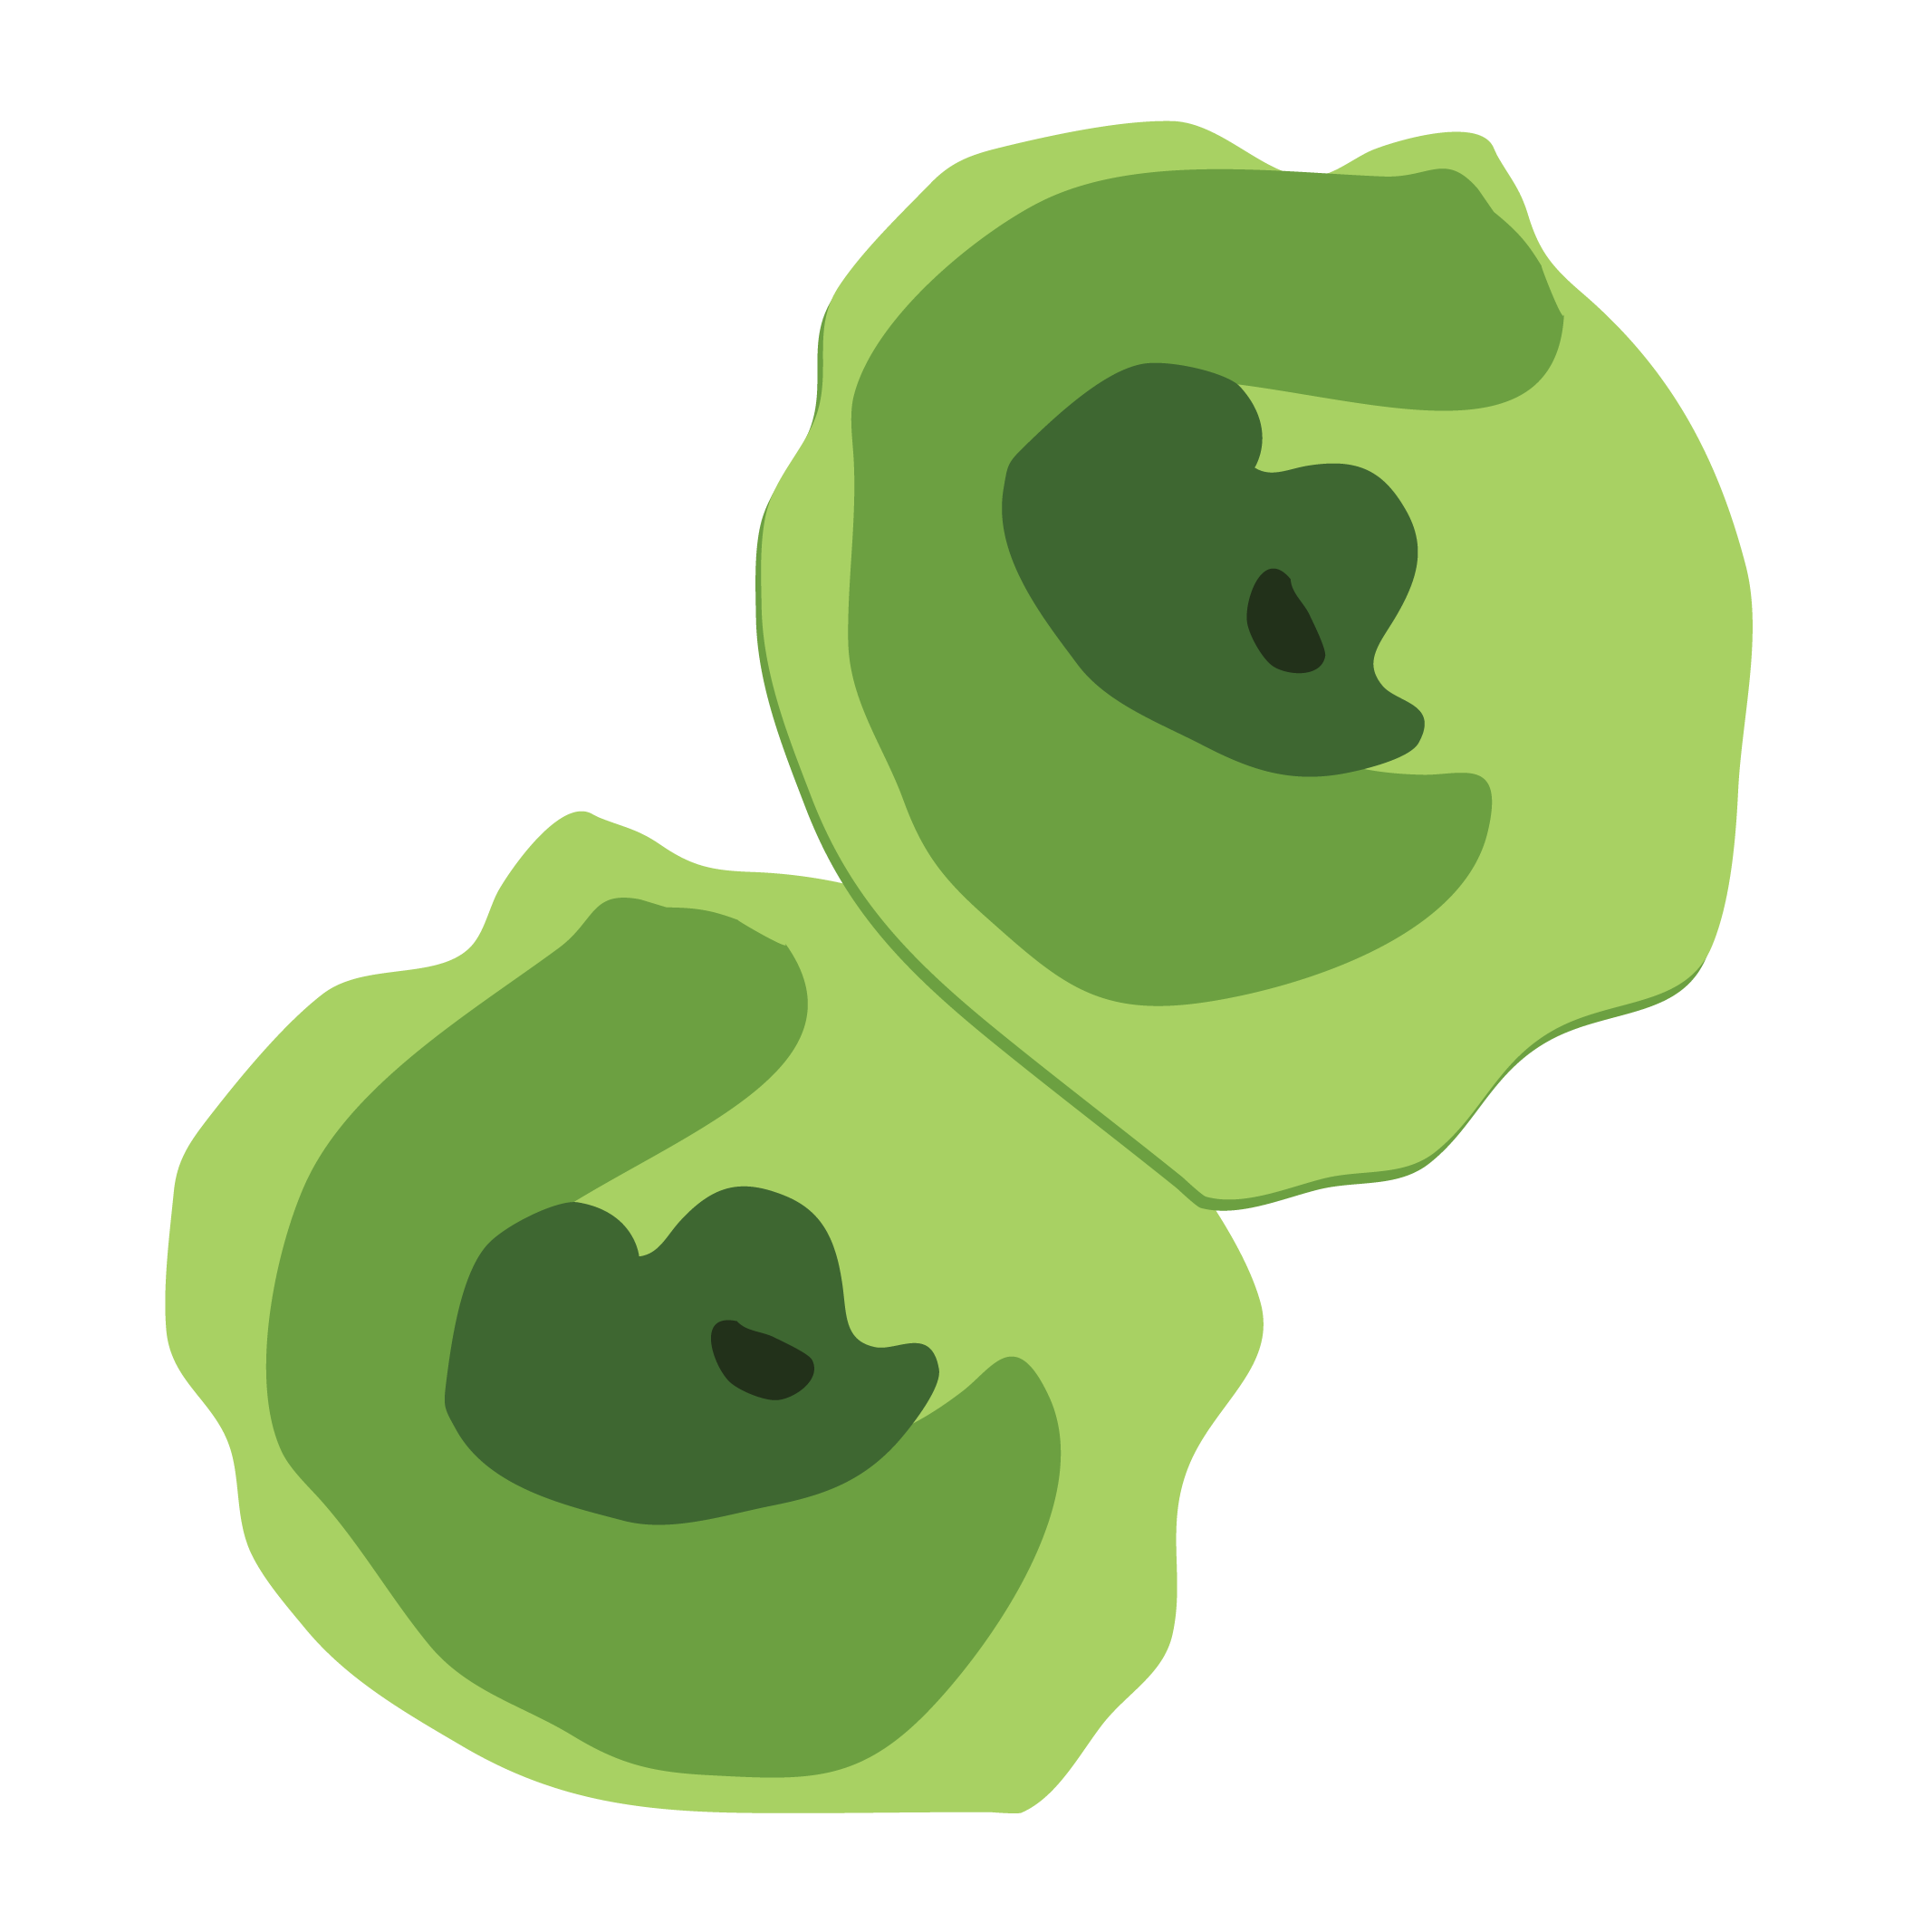
\includegraphics[valign=m,scale=0.1]{images/species_05.png} & Sir Guava & Green Cheecks Busheeks & Peapod \\ 
Species 6  & 
\includegraphics[valign=m,scale=0.1]{images/species_06.png} & Spotted Ninja & SquidWard & Miranda Sings \\ 
Species 7  & 
\includegraphics[valign=m,scale=0.1]{images/species_07.png} & Mello Jello & Sumbraro & Egg \\ 
Species 8  & 
\includegraphics[valign=m,scale=0.1]{images/species_08.png} & Majigger & Miranda Sings & Froggy Thingy \\ 
Species 9  & 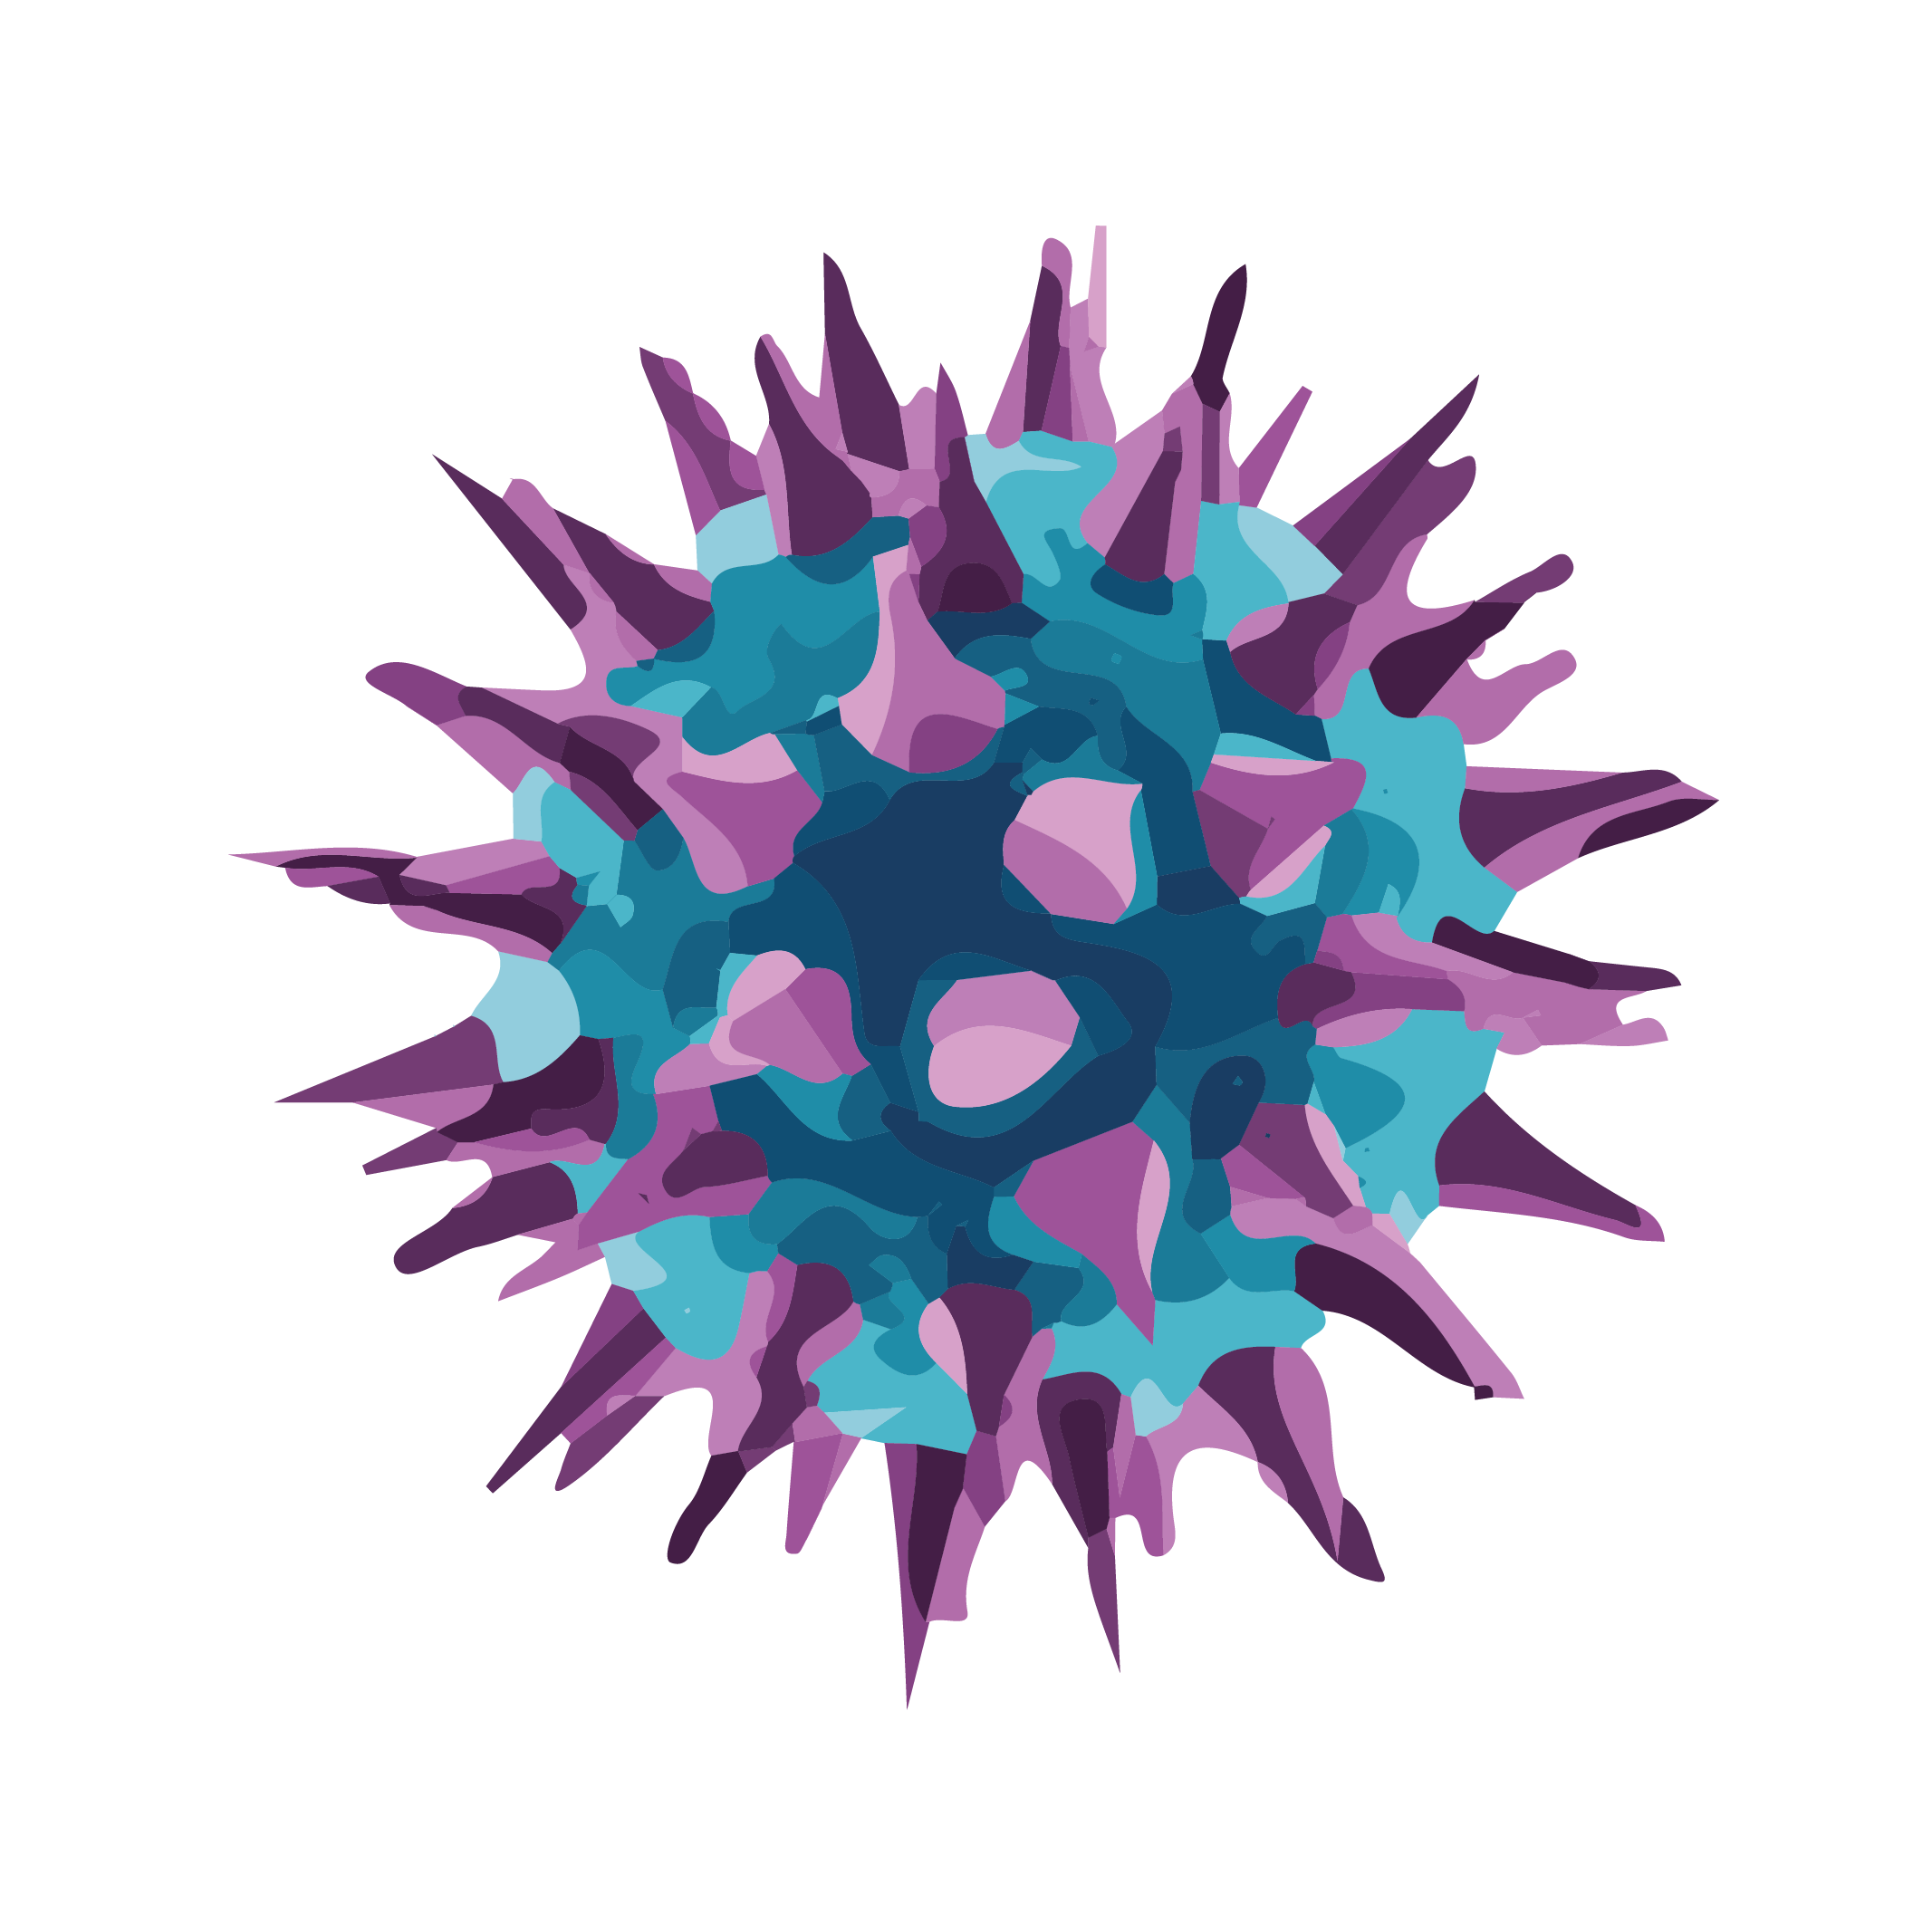
\includegraphics[valign=m,scale=0.1]{images/species_09.png} & Spikeface & Ouch & Spike \\ 
Species 10 & 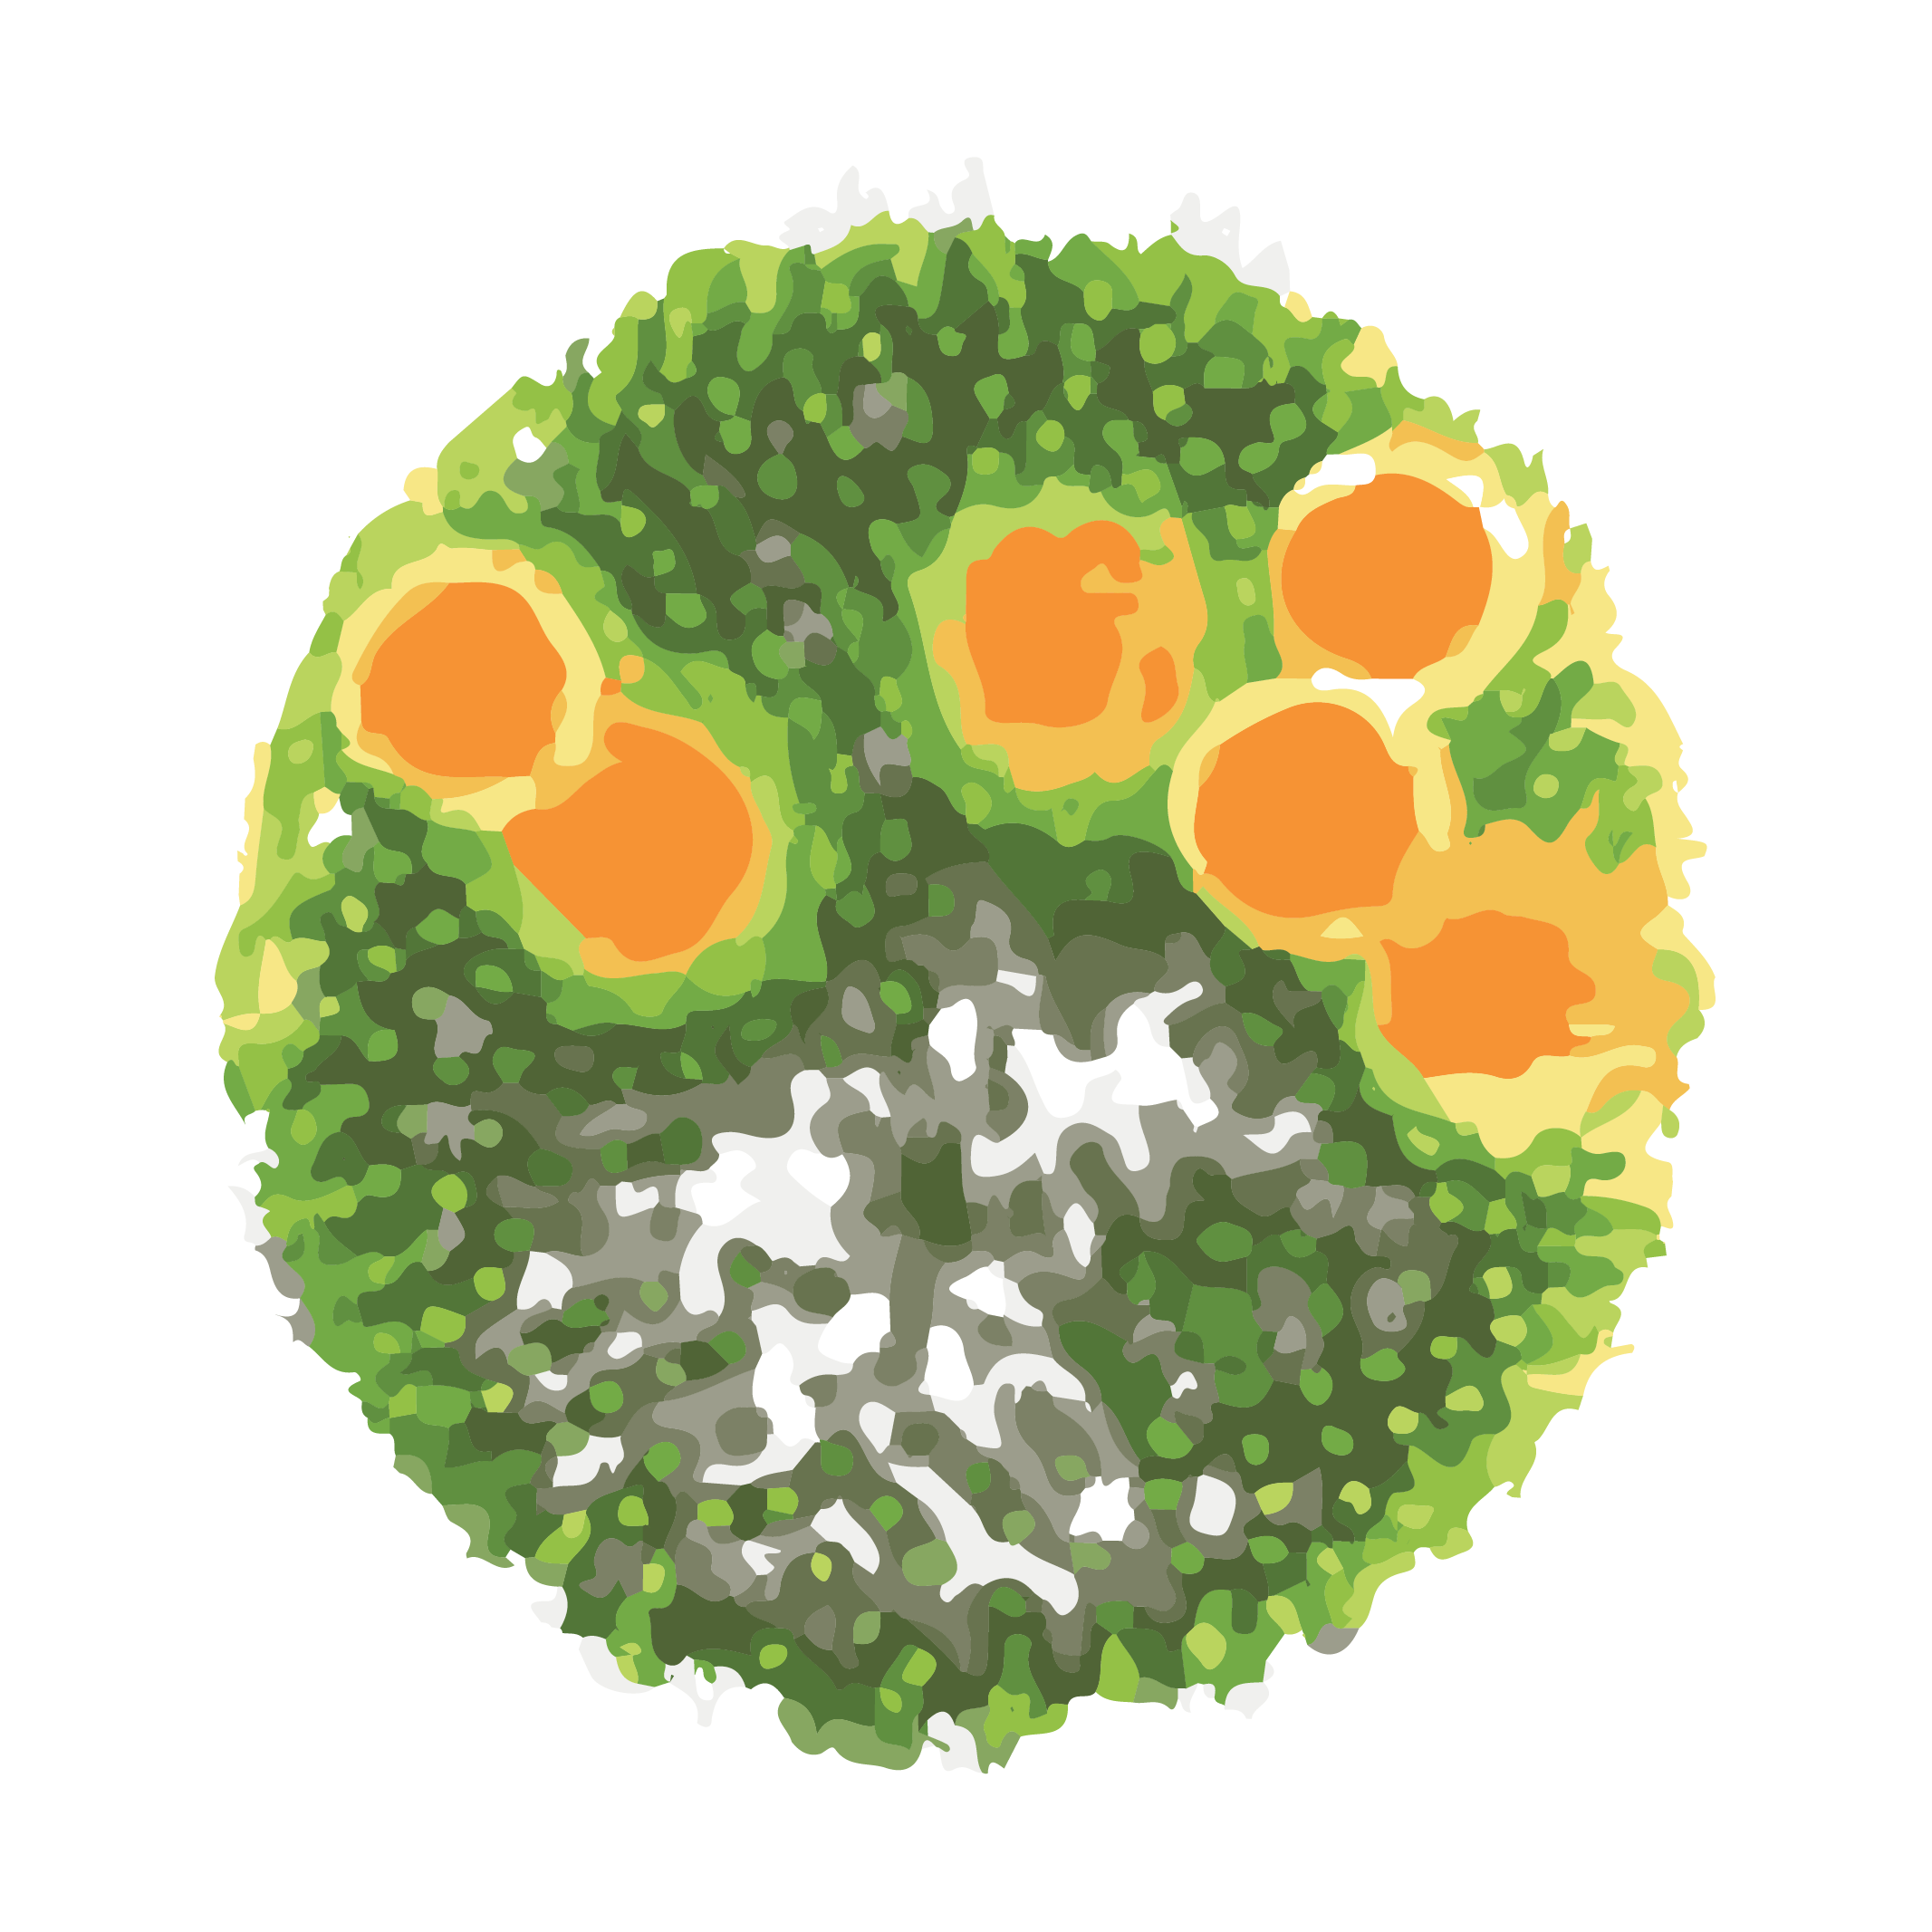
\includegraphics[valign=m,scale=0.1]{images/species_10.png} & Su-Shay & Salad & Chez Bai \\ 
\hline
\end{tabular}
\label{tab:species_names}
\end{table}

In the questionnaire, 33/46 students preferred this kind of interface over the conventional \textit{Graphical User Interface} (implemented as web interface in this study), despite the fact that using it is more time consuming. 4/46 prefer not to use it, because clicking on a screen is faster and more efficient and the others don't have any preference. In the open questions, the word "fun" was mentioned 42 times (second only to "tangibles" with 57 mentions) and "cool" 20 times. Analyzing the semantics of the explanations, 36 students think that having tangibles is great for creating a fun atmosphere in class and "makes this project even more fun". When asked if they suggest to use the tangibles in the future, 37/46 students answered positively with strong arguments supporting tangibles, 5/46 thought that is better not to use them because they are a waste of time (e.g. waiting in line for others to return them) or because sometimes they had difficulties at the beginning on understanding how to execute an action. An interesting argument (shared by 4 students across all the three classes) is that children don't understand immediately how they works and they are excited and curious about what happens behind the scenes.
\begin{quote}
\textit{[Questionnaire]
I think the tangibles are a good way to get kids excited about learning, since they seem like magic, even though I know that there is a chip of some sort in them.}
\end{quote}
From video sources it is possible to understand that many children were also interested to the technology that make them work because they never saw something similar before. An example that I want to report is a student that placed his hand on top of the iPad in order to see what outcome the system will produce, waiting for few seconds and asking why his hand was not tracked like a tangible. Tools like this can be used in order to make children engaged with general science and develop an interest in computer science.
\begin{quote}
\textit{[Questionnaire]
Use the tangibles because kids will think something like "wow it's magic"}
\end{quote}

Lastly I would like to report that students really appreciated the quality of the tangibles that are a high fidelity reproduction of creatures contained in the computer graphic simulation. Most of them looked at all the creatures’ details before even start using them for the classroom activity.
\begin{quote}
\textit{[Questionnaire]
The tangibles teach us the looks of the creatures because I had no idea what the underside of the creatures.}
\end{quote}
Students were truly inspired by their look and feel, other than expressing verbally their comments they wanted to write them down in the questionnaire:
\begin{quote}
\textit{[Questionnaire]
[...] not only is it lots more fun and interesting, it shows just what a 3-D printer can do!}
\end{quote}

\begin{quote}
\textit{[Questionnaire]
[I like] the tangibles because it's very creative}
\end{quote}

The answer to the first part of the \textit{second research question} is that tangibles can motivate students. During this study, as explained in this section, I found evidence that keeping students engaged into fun and enjoyable activities adds motivational value for the students. 

Collected data also suggest that tangibles have properties of \textit{cultural artifacts} \cite{horn:role}:
\begin{itemize}
\item They activate social resources learned way before starting using them: how to share a toy with other children.
\item Peers taught each other strategies to use them taking advantage of their social skills.
\end{itemize}
The model used for introducing species into habitats (get tangibles close to computer where the habitat is simulated) was not immediately recognized and for this reason they are not \textit{social signifiers} \cite{norman:way}. For this reason I argue that tangibles in this case are not cultural artifacts (even if they present some properties of them). This is the answer to the last part of the second \textit{research question} and gives also a clue on how to better improve tangible interaction in the future for taking full advantage of \textit{cultural artifacts} \cite{horn:role} capabilities that comes with them. 

\subsection{How one set of tangibles helps students to discuss}
Evidence in the video suggest that introducing limited resources (one set of tangibles) that must be used by all the groups creates great opportunities for discussion about the scientific topic of the lecture between children of the same group and also between children in different groups.

This is a behavior that I expected when I described the opportunities that tangibles creates and is the answer the second part of the \textit{second research question}. In this subsection I describe it in details. It was easy to anticipate this behavior, because forcing children to have limited resources naturally creates a place where they have to wait for them to became available.

Perturbation to the habitats, the only activity that required tangibles, was often executed as last activity of the lesson in 15 or 20 minutes of time. Before perturb the habitat every group had to make a proposal and a prediction of the outcome. After the proposal they had to go in the middle of the room, take the tangibles and return to their habitat for executing the action placing the tangible near the iPad. If the tangibles were not available the adopted solutions were two:
\begin{itemize}
\item Go to the the group that owned the needed tangible and ask the permission to be the next to use it.
\item Remain at the central table and discuss with the other students while waiting the desired tangible to became free.
\end{itemize}
Usually for every group only two or three students went to the central table for taking the tangibles, it was rare that the entire group did it.

Students of that classes never used a tangible interface before, this fact encouraged at the beginning discourses on how to use them more than productive didactic discourses. Not every one understood how they works (e.g. they must be placed near the habitat) and they sought the help of classmates. Passed the first lesson discourses became more productive almost exclusively about the action that they wanted to perform on their environment. In the questionnaire 14/46 students admitted to have at least one productive discourse with other groups confirming video evidence:
\begin{quote}
\textit{[Questionnaire]
We mostly talked about what was going on in our ecosystems but we asked some of the other groups what changes they were making.}
\end{quote}

Another positive, interesting and unattended behavior is that students could hear other groups conversations since they were concentrated around the same table, also without a direct interaction:
\begin{quote}
\textit{[Questionnaire]
We talked about it a little bit [perturbation of our habitat] and heard the other groups plans. We all rushed to get the tangibles though I didn't really get to have a conversation.}
\end{quote}
This is also an evidence that the social protocol used for accessing the data was \textit{First to Take First to Use}. There are no sign of disputes between students. The teacher never had to intervene for stopping inappropriate behaviors.
\begin{quote}
\textit{[Questionnaire]
There was a line and we had to wait for them to check ours before we did it.}
\end{quote}

All the behaviors described were positives and contributed to social interaction, free discussion and knowledge exchange, but 15/46 students perceived having only one set of beacons as a problem often identifying the waste of time as an issue for them.
\begin{quote}
\textit{[Questionnaire]
It took a little more time because some groups needed the same tangible.}
\end{quote}
\begin{quote}
\textit{[Questionnaire]
I think that we should not use tangibles next year because they are unnecessary and waste class time. When you put them on the iPad, there can be a delay and it makes us unable to complete certain things.}
\end{quote}

Another interesting and unexpected fact discovered is that children tend to copy the actions of other groups. As shown in \ref{tab:perturbations} there are cases in which the choice of species is not random, for example in perturbation 3 one class chose only species 8 and 10. Evidence supporting this claim are present also in the questionnaire:
\begin{quote}
\textit{[Questionnaire]
In waiting we had an opportunity to discuss with others ecosystems. Also, without even talking, you could see what other ecosystems were doing with a cursory glance.}
\end{quote}

\begin{table}
\centering
\caption{PERTURBATIONS APPLIED TO HABITATS}
\begin{tabular}{ | l | l | l | l | l | l | }
\hline
Perturbation \# & Class  & Habitat \# & Action & Species & Interface \\
\hline
\hline
\multirow{12}{*}{Perturbation 2} & \multirow{4}{*}{6A} & habitat 1 & Decrease  & Species 8 & Web \\
 & & habitat 2 & Increase & Species 8 & Web \\
 & & habitat 3 & Increase & Species 1 \& 2 & Web \\
 & & habitat 4 & Increase & Species 7 & Web \\
\cline{2-6}
 & \multirow{4}{*}{6B} & habitat 1 & Increase & Species 10 & Web \\
 & & habitat 2 & Increase & Species 9 & Web \\
 & & habitat 3 & & & Web \\
 & & habitat 4 & Increase & Species 7 & Web \\
\cline{2-6}
 & \multirow{4}{*}{6C} & habitat 1 & Decrease & Species 10 & Tangible \\
 & & habitat 2 & Increase & Species 0 & Tangible \\
 & & habitat 3 & Increase & Species 1 & Tangible \\
 & & habitat 4 & Decrease & Species 7 & Tangible \\ 
\hline
\multirow{12}{*}{Perturbation 3} & \multirow{4}{*}{6A} & habitat 1 & Decrease & Species 2 & Tangible \\
 & & habitat 2 & Increase & Species 7  & Tangible \\
 & & habitat 3 & Increase & Species 10 & Tangible \\
 & & habitat 4 & Decrease & Species 10 & Tangible \\
\cline{2-6}
 & \multirow{4}{*}{6B} & habitat 1 & Decrease & Species 8 & Tangible* \\
 & & habitat 2 & Decrease & Species 8  & Tangible* \\
 & & habitat 3 & Decrease & Species 10 & Tangible* \\
 & & habitat 4 & Decrease & Species 10 & Tangible* \\
\cline{2-6}
 & \multirow{4}{*}{6C} & habitat 1 & Decrease & Species 8 & Tangible \\
 & & habitat 2 & Increase & Species 7 & Tangible \\
 & & habitat 3 & Increase & Species 3 & Tangible \\
 & & habitat 4 & Decrease & Species 7 & Tangible \\ 
\hline
\multirow{12}{*}{Perturbation 4} & \multirow{4}{*}{6A} & habitat 1 & Insert & Species 7 & Tangible \\
 & & habitat 2 & Insert & Species 1 & Tangible \\
 & & habitat 3 & Insert & Species 0 & Tangible \\
 & & habitat 4 & Insert & Species 1 & Tangible \\
\cline{2-6}
 & \multirow{4}{*}{6B} & habitat 1 & Insert & Species 7 & Tangible \\
 & & habitat 2 & Remove & Species 4 & Tangible \\
 & & habitat 3 & Insert & Species 7 & Tangible \\
 & & habitat 4 & Insert & Species 1 & Tangible \\ 
\cline{2-6}
 & \multirow{4}{*}{6C} & habitat 1 & Remove & Species 8 & Tangible \\
 & & habitat 2 & Remove & Species 9 & Tangible \\
 & & habitat 3 & Insert & Species 2 & Tangible \\
 & & habitat 4 & Insert & Species 9 & Tangible \\ 
\hline
\end{tabular}
\label{tab:perturbations}
\end{table}

From this story I can gather the answer for the second part of the \textit{second research question}: creating a bottleneck at the central table (where everyone have to take the tangibles) creates an unique place inside the classroom where students can exchange information while waiting and lead to productive discourses about the scientific topic.

\subsection{Feeling more in control and minimize the errors}
I found evidence that children feels more in control of the changes when they use tangibles. In WallCology application the changes applied to ecosystems are extremely important for the outcome of the experiment and students were totally aware of it. Introducing a new species or removing an existing one can have devastating consequences on the populations living in the habitats. For this reason the interface that allow them to modify critical parameters must be designed keeping in mind the error minimization principle \cite{norman:design}. The web interface implements this principle displaying a message asking for a confirmation before applying any change, nevertheless young students didn't feel enough in control because they perceive the affordance \cite{norman:affordance} of irreparably destroy their ecosystem with two clicks (one on the action and one on the confirm button). Tangibles expose a different set of properties that minimize the error possibility requiring locomotion in order to apply changes to the habitat. The evidence can be found in the questionnaire:
\begin{quote}
\textit{[Questionnaire]
I like having tangibles because I think it's easier to focus and concentrate when I'm in control of what I'm doing. [...]}
\end{quote}

\begin{quote}
\textit{[Questionnaire]
I think that it's pretty cool to have tangibles, because whereas the computer is doing everything, you feel like you have more control of your habitat while placing the tangibles on the iPad. I feel this because it's nice to see a practical demonstration of what's going to happen; Chez Ball decreases, Sorbet increases, etc. [...]}
\end{quote}

\begin{quote}
\textit{[Questionnaire]
Because it's easier to visually see what you're actually doing [while using tangibles] and you can't accidentally click the wrong thing.}
\end{quote}

Evidence of mistakes committed by students while using the web interface for executing the second perturbation are present in the application log. Two groups wrongly executed two actions instead of one and one group didn't complete the action the first day (\ref{tab:perturbations}). Group three in 6A increased both species 2 and species 1 and group four increased twice species 7. This kind of errors were not present while they were using the tangible interface because only one modification every 30 seconds was allowed by the interface.

Based on the error evidence other two mechanisms were designed and implemented for improving the usability of the \textit{population control} interface:
\begin{itemize}
\item \textit{Backend input verification system}: it didn't allow more than one consecutive action of the same type on the same species for the same habitat. An error message is also sent to the front end in case the rule is violated (the interaction is logged anyway).
\item \textit{Action executed with success message}: in order to give feedback \cite{norman:design} to the user and be sure that the system successfully register the changes.
\end{itemize}

At this point I listed the evidence necessary to answer the \textit{first research question} and explain how teachers and learners coordinate their use of shared tangibles in this study. Tangibles were left on the central table without any form of control imposed by teachers. Students of all the three classes were able to coordinate the access to the tangibles without problems, following the social protocol \textit{First to Take First to Use} that creates a line and some minutes of waiting time at the central table. Some students decided not to wait in line and went directly to other groups in order to ask the needed tangible, missing the opportunity to discuss with other students, but discovering the perturbation that the other group was applying.

\section{Summary and research results}

It is difficult to assert if tangibles help students to learn, but I found evidence of behaviors that are commonly considered good practice for learning inside the school. Those behaviors are summarized in:
\begin{itemize}
\item Engage the students in fun and glad activities.
\item Inspire curiosity and creativity.
\item Face to face conversations and talks about a scientific inquiry.
\item Discussions and information sharing between different groups while waiting their turn of using tangibles.
\item Know what other groups are doing.
\item Empathy with the creatures and a more personal connection with them.
\end{itemize}

In this study the students were left without teacher control. They were able to autonomously coordinates in order to use the tangibles to accomplish the assigned goal of applying perturbations to the ecosystems. As a result, interactions between students increased in number and were not only focused on the material actions for achieving the goal, but were also about the science domain behind the simulation. Shared control tangibles definitely create opportunities for engaging students in discussions, not possible with classical user interfaces (answer to the second research question of this study). Those discussions were possible because of the competition for having those limited resources and they created no disputes between students. The outcome of this study is overall positive and provides evidence that tangible interfaces are mature enough for being employed in real classes. 

The obtained results also confirms that \textit{RoomPlaces} is able to support those activities making it an essential tool in this research and highlighting its effectiveness in a real use case scenario. \textit{RoomPlaces} was robust enough for supporting 60 uninterrupted days of running concurrently in three different classes without any crash of its components and it required no external intervention for fixing errors during the study (thanks also to the previous six months of lab testing). It was used by researchers other than me that received no training on how to use it other than simple high level instructions that can be easily executed by teachers with no specific competences. During the study, many functions of \textit{RoomPlaces} were not required leaving some open question about their effectiveness and robustness in real case scenarios.
